\documentclass{article}

\usepackage[margin=1in, top=1.5in, bottom=1.5in, columnsep=0.25in]{geometry}
\usepackage{multicol}
\usepackage{graphicx}
\usepackage{hyperref}
\usepackage{amsmath}
\usepackage{float}
\usepackage{siunitx}
\usepackage{tikz}
\usepackage{subcaption}
\usepackage{mathtools} 
\usepackage[backend=biber, sorting=none]{biblatex}

% \usepackage{amssymb}
% \usepackage{marvosym}
% \usepackage[all]{hypcap}
% \usepackage[linesnumbered,ruled,vlined]{algorithm2e}
% \usepackage[framed, numbered]{matlab-prettifier}
% \usepackage{courier}

\counterwithin{figure}{section}
\counterwithin{equation}{section}
\counterwithin{table}{section}

\addbibresource{references.bib}

% \DeclareMathOperator*{\argmin}{arg\,min}

\title{\large Project of \textit{Control Problems in Robotics} \\ 
\LARGE Modeling and controlling the Mars Helicopter \textit{Ingenuity}}
\author{Davide De Santis \\1886037\\ \textit{DIAG Department}\\ \textit{University of Rome “La Sapienza”}\\desantis.1886037@studenti.uniroma1.it
\and Simone Orelli\\1749732\\ \textit{DIAG Department}\\ \textit{University of Rome “La Sapienza”}\\orelli.1749732@studenti.uniroma1.it 
\and Antonio Rapuano\\2044902\\ \textit{DIAG Department}\\ \textit{University of Rome “La Sapienza”}\\rapuano.2044902@studenti.uniroma1.it
\and Mert Tekyurt\\2057350\\ \textit{DIAG Department} \\ \textit{University of Rome “La Sapienza”}\\tekyurt.2057350@studenti.uniroma1.it}
\date{April 2024}


\begin{document}
    \maketitle
    \thispagestyle{empty}
    \begin{multicols}{2}
    \begin{abstract}
    This paper details the process of developing a control system for Ingenuity, a drone helicopter that operated from 2021 to 2024 on Mars as part of NASA's Mars 2020 mission. Said process consists first of creating a mathematical model capable of representing the behavior of the drone in flight over Mars, and then designing a controller capable of imparting desired behavior and performance (trajectory tracking) to the model. 
    The problem is approached through two different control strategies: first, with a static input-to-output feedback linearization controller, and then, through the backstepping technique. Among the two, only the latter returns satisfactory results, as it is able to achieve the objectives by exploiting the fact that Ingenuity is an underactuated robot.
\end{abstract}
    \vfill\null
    \columnbreak

    \tableofcontents

    \newpage
    \setcounter{page}{1}
    
    \section{Introduction}
A fully-actuated (or even redundant) robot is capable of performing operations and accomplishing tasks with extreme accuracy and repeatability. On the other hand, when the number of actuators is less than the number of degrees of freedom, the capabilities of the robot are reduced, and it is said to be underactuated. \\
Underactuation is not only a hurdle, but it brings a whole host of advantages, first and foremost efficiency (but also spectacularity) both in design and operation, although this comes at the cost of severely complicating their control.

A widely-used class of optimal control algorithms that allows good trajectory tracking performance of systems with a high degree of nonlinearity such as underactuated robots is that of Differential Dynamic Programming (DDP) methods. Introduced in 1966 by Mayne \cite{mayne}, they can be exploited to implement a receding-horizon control strategy reminiscent of Model Predictive Control \cite{tassa07}. The optimal control problem to be solved can also embed input constraints, which are common in robotics applications \cite{tassa14}. 

This document addresses the implementation of a controller for two among the most significative examples of underactuated robots, namely the pendubot and the acrobot. For robustness concerns, DDP is used to find optimal trajectories continuously in real-time according to a receding horizon logic, in the meantime satisfying hard constraints on the control sequence. The performance of the controller is evaluated through simulations, and then the results are discussed.
    \section{Mathematical model}
Each of the two rotors of Ingenuity generates a thrust vector in a commanded direction, which is applied on the rotating hub. Not only does this result in a force capable of moving the helicopter, but it also generates a torque that can be used to control its orientation. \\The helicopter is treated as a simple rigid body without taking into account the aerodynamics of the blades, therefore the only external force is gravity. 

From now on, we will consider an inertial reference frame (superscript $^i$) and a non-inertial one attached to the drone body (superscript $^b$). \\ The relative orientation of the latter with respect to the former is expressed in roll, pitch and yaw angles (i.e. the three components of $W$), or alternatively through the corresponding rotation matrix (in compact trigonometric notation with $\sin(W_i) = s_i$ and $\cos(W_i) = c_i$):
\begin{align*}
    R(W) = R = \begin{bmatrix}
        c_2 c_1& s_2 s_1 c_3 - s_1 c_3 & s_3 s_2 c_1 + s_1 s_3 \\
        c_2 s_3 & s_2 s_1 s_3 + c_3 c_1 & s_3 s_2 c_1 - s_1 c_3 \\
        -s_2 & s_1 c_2 & c_2 c_1
    \end{bmatrix}
\end{align*}

\subsection{Helicopter dynamics}
The magnitude of the thrust generated by each of the rotors is given by the sum of two components, one due to the lift and the other due to the drag. 
\begin{gather*}
    F_l = K_l \omega^2, \\
    F_d = K_d \omega^2,
\end{gather*}
where $\omega$ represents the angular velocity of the rotor, while $K_l$ and $K_r$ are two coefficients, whose expressions are the following:
\begin{gather*}
    K_l = \frac{1}{2} C_l c r^3 \rho, \\
    K_d = \frac{1}{2} C_d c r^3 \rho.
\end{gather*}
In the previous formulas, $c$ is the chord of a rotor blade and $r$ is its hub-to-tip length; $\rho$ is the air density, while $C_l$ and $C_d$ indicate the lift and drag coefficients of the rotor blades, which depend on their angle of attack. We consider the latter constant at a value such that $K_l - K_d > 0$.\\
This means that we can write the total thrust norm generated by each rotor as:
\begin{gather}
    ||F|| = F_l - F_d = (K_l - K_d) \, \omega^2, \label{eq:force_norm}
\end{gather}
therefore we can treat $\omega_u$ and $\omega_l$ as two of the control inputs of the system (respectively, for the upper and lower rotor).

Now consider the angles that the projections of the thrust vectors on the planes $xz$ and $yz$ form with the vertical axis $z$, called respectively $\alpha$ and $\beta$: this couple is the other input of the system, and it is the same for the upper and lower rotors. The two angles are illustrated in Figure \ref{fig:alpha_beta}.

\begin{figure}[H]
    \centering
    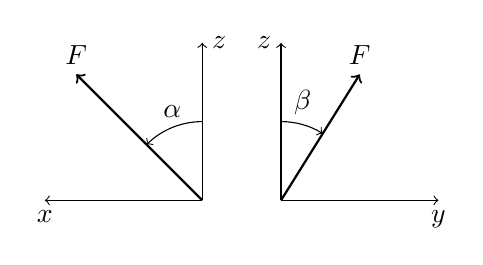
\begin{tikzpicture}[scale=2]
        \draw[->] (0,0) -- (0,1) node[right] {$z$};
        \draw[->] (0,0) -- (-1,0) node[below] {$x$};
        
        \draw[->,thick] (0,0) -- (-0.8,0.8) node[above] {$F$};
        
        \draw[->] (0,0.5) arc (90:135:0.5) node[midway, above] {$\alpha$};

        \draw[->] (0.5,0) -- (0.5,1) node[left] {$z$};
        \draw[->] (0.5,0) -- (1.5,0) node[below] {$y$};
        
        \draw[->,thick] (0.5,0) -- (1,0.8) node[above] {$F$};
        
        \draw[->] (0.5,0.5) arc (90:58:0.5) node[midway, above] {$\beta$};
    \end{tikzpicture}
    \caption{Angles $\alpha$ and $\beta$ that the projections of the thrust vector forms with the vertical direction in the $xz$ and $yz$ planes of the body frame.}
    \label{fig:alpha_beta}
\end{figure}

\noindent In the body reference frame, the thrust vector is then written by means of the auxiliary angle $\gamma$, i.e. the angle that the thrust vector forms with the vertical axis $z$ in the three-dimensional space:
\begin{align}
    F^b = T_{(\alpha, \beta)}||F|| \label{eq:force}
\end{align}
\vspace*{-0.6cm}
\begin{align*}\text{with} \quad T_{(\alpha, \beta)} = \begin{bmatrix}
        -\tan{\alpha} \cos{\gamma} \\
        -\tan{\beta} \cos{\gamma} \\
        \cos{\gamma}
    \end{bmatrix}, \\
    \tan^2{\gamma} = \tan^2{\alpha} + \tan^2{\beta}. 
\end{align*}

Since the thrust vectors are not applied in the center of mass of the helicopter, they also generate torques according to:
\begin{align} 
    \tau^b = \begin{bmatrix}
        0 \\ 0 \\ d_{cm}
    \end{bmatrix} \times F^b, \label{eq:torque_due_force}
\end{align}
with $d_{cm}$ being the distance between the center of mass of the helicopter and the center of the rotors.\\
Note that this cross product results in a vector whose last component is null. In fact, the yaw rotation is caused by the difference of the reaction torques generated by the two rotors:
\begin{align} 
    \tau^b_r = \begin{bmatrix}
        0 \\ 0 \\ Q_u - Q_l
    \end{bmatrix} \quad \text{with} \quad Q = 0.02 \; ||F||. \label{eq:reaction_torque}
\end{align}

According to Newton's second law, the overall force acting on the helicopter is the sum of the forces generated by the two rotors and the force of gravity:
\begin{gather*}
    \begin{split}
        F^b_{tot} & = F^b_u + F^b_l + R^T F^i_g \\
        & = T_{(\alpha, \beta)} (K_l - K_d) (\omega^2_u + \omega^2_l)+ R^T F^i_g,
    \end{split}
\end{gather*}
where \(F^b_{tot}\) is the total force acting on the body and \(F^i_{g}\) is the gravitational force.
Similarly, the total torque is composed of the torques generated by the two rotor thrust vectors (roll and pitch) and the reaction torque of the two rotors (yaw):
\begin{align}
    \tau^b_{tot} = \tau^b_u + \tau^b_l + \tau^b_r,
    \label{eq:torque}
\end{align}
where $\tau_{tot}^b$ is the total torque acting on the body.

By applying these laws, we compute the derivative of the velocity $V$ in the body frame. Neglecting external forces, the cross product term accounts for the Coriolis effect.
This is also done for the angular velocity $\Omega$, where the cross product term represents the gyroscopic effect.
\begin{gather*}
    \frac{d}{dt}{V^b} = \frac{F^b_{tot} - \Omega^b \times (m V^b)}{m}, \\
    \frac{d}{dt}{\Omega^b} = I^{-1} (\tau^b_{tot} - \Omega^b \times (I \Omega^b)).
\end{gather*}
In the inertial frame, the position $P$ and the orientation $W$ of the robot are updated by integrating the velocity and the angular velocity, with:
\begin{gather*}
    \frac{d}{dt}P = R\, V^b, \\ 
    \frac{d}{dt}W = R\, \Omega^b.
\end{gather*}
\subsection{Actuator dynamics}
The control signals $\omega_u$, $\omega_l$, $\alpha$ and $\beta$ are not instantly translated into the corresponding angular velocities or swashplate tilt angles: non-idealities arise since the physical components of Ingenuity are set in motion by actuators (typically electrical motors). \\
In reality, often actuators integrate low-level closed loops (sometimes even analog, e.g. through potentiometers) whose dynamics may be overlooked in the high-level control system design.
To account for the effect of these components in our model and simulations, however, it is appropriate to model each of the four input channels as double integrators:
\begin{align*}
    G_i(s) = \frac{1}{s^2}, \quad i = 1, 2, 3, 4.
\end{align*}
In feedforward, the trivial solution is to control the double integrators with (physically realizable) controllers such as:
\begin{align*}
    K_i(s) = \frac{s^2}{(1 + s \, T_i)^2}, \quad i = 1, 2, 3, 4,
\end{align*}
with $T_i$ being a (small enough) time constant that can be tuned to match the actual dynamics of the actuators. \\
This means that, at the end of the day, the resulting actuator open-loop transfer functions are equal to:
\begin{align*}
    L_i(s) = G_i(s) \, K_i(s) = \frac{1}{(1 + s \, T_i)^2}, \quad i = 1, 2, 3, 4.
\end{align*}
    \section{Control via I/O feedback linearization}
From the control perspective, Ingenuity is an underactuated robot, since the number of control inputs is less than the number of degrees of freedom. Specifically, it has six degrees of freedom (three for the position and three for the orientation) and only four control inputs (the rotation speed of the two rotors $\omega_u$ and $\omega_l$, and the thrust vector angles $\alpha$ and $\beta$). 

In order for the robot to be controlled, it is necessary to exploit its natural dynamics by employing the four inputs  to impart a certain behavior to the total system (both positional and rotational state variables) such that, at the end of the day, the three-dimensional position and the yaw angle follow the desired course in time. To grasp the concept, the reader can imagine a quadrotor or helicopter with a tail rotor, which need to tilt in the desired direction in order to move.

If we choose as controlled outputs of the system the three position components and the yaw angle, it is possible to employ the input-to-output feedback linearization technique to design a controller that renders unobservable the nonlinear dynamics of the helicopter. As a result, the system seen between input and output will have linear dynamics and thus could be easily controlled via linear control techniques.

Consider the following nonlinear state-space representation of the robot dynamics:
\begin{align}
    \frac{d}{dt} \begin{bmatrix}
        P \\ V^b \\ W \\ \Omega^b
    \end{bmatrix} = \begin{bmatrix}
        R \, V^b \\ \frac{1}{m} R^T F_g^i -\Omega^b \times V^b + \frac{1}{m} u \\ R \, \Omega^b \\ -I^{-1} \Omega^b \times (I \Omega^b)+I^{-1}\tau_{tot}^b 
    \end{bmatrix}
    \label{eq:fbl_model}
\end{align}
where the input $u$ is the total thrust force generated by the rotors: 
\begin{align}
    u = F_u^b + F_l^b.    
    \label{eq:u} 
\end{align}
Calculations are facilitated if we make a change of coordinates to the inertial frame. 
$$ \frac{d}{dt} \begin{bmatrix}
    P \\ \dot{P}
\end{bmatrix} = \begin{bmatrix}
    \dot{P} \\ \frac{1}{m} F_g^i + \Omega^b \times \dot{P} - (R \Omega^b) \times \dot{P} + \frac{1}{m} R u
\end{bmatrix}. $$

The idea is to choose $u$ to cancel the nonlinear part of the positional dynamics:
$$u = m R^T [(R \Omega^b) \times \dot{P} - \Omega^b \times \dot{P} - \frac{1}{m} F_g^i + v].$$
The transfer function relating the input $v$ to the output $P$ is then a double integrator:
$$\frac{d^2}{dt^2} P(t) = v(t) \iff \frac{P(s)}{v(s)} = \frac{1}{s^2}.$$
It can be controlled using a simple PD controller with a feedforward term:
$$v = k_{p,1} (P_d - P) + k_d \bigg(\frac{d}{dt}P_d - \dot{P}\bigg) + \frac{d^2}{dt^2}P_d.$$

Notice that the only input affecting the $\Omega_3^b$ dynamics is the reaction torque $\tau_r^b$. Controlling the third component of the angular velocity in the body frame is all we can do if we want to keep the inputs $u$ and $\tau_r^b$ decoupled, and it is sufficient if we assume that the roll and pitch angles are sufficiently small. Therefore, we proceed in an analogous way to the previous case, choosing:

$$ \tau_r^b = \begin{bmatrix}
    0 & 0 & 0 \\ 0 & 0 & 0 \\ 0 & 0 & 1
\end{bmatrix}[\Omega^b \times (I \Omega^b) + I w]$$
This results in the following transfer function for the $\Omega_3^b$ dynamics:
$$\frac{d}{dt} \Omega_3^b(t) = w_3(t) \iff \frac{\Omega_3^b(s)}{w_3(s)} = \frac{1}{s},$$
where $w_3$ is the third component of $w$. The linearized system can be controlled using a simple proportional controller with a feedforward term:
$$w = \begin{bmatrix}
    0 \\ 0 \\k_{p,2} (\Omega_{3,d}^b - \Omega_3^b) + \frac{d}{dt}\Omega_{3,d}^b
\end{bmatrix} .$$

Following this, a critical point is reached: once an feedback linearizing control is implemented, it is worth taking a look at how the part of the system that has been hidden behaves. We could call this part, in a non-formal way, the \textit{forced zero dynamics} of the system. It is obtained by substituting \ref{eq:torque_due_force} and \ref{eq:torque} in \ref{eq:fbl_model}:
\begin{align*}
    \frac{d}{dt}\begin{bmatrix}
        \Omega^b_1 \\
        \Omega^b_2
    \end{bmatrix}
    = 
    \begin{bmatrix}
        -\frac{F_{l,2}^b d_{cm,l} + F_{u,2}^b d_{cm,u}}{I_{1,1}} - \frac{I_{2,2}-I_{3,3}}{I_{1,1}} \Omega^b_2 \Omega^b_3 \\
        \frac{F_{l,1}^b d_{cm,l} + F_{u,1}^b d_{cm,u}}{I_{2,2}} + \frac{I_{1,1}-I_{3,3}}{I_{2,2}} \Omega^b_1 \Omega^b_3
    \end{bmatrix}.
\end{align*}
The latter is an autonomous dynamics that is affected by the signals $F_{l,1}^b$, $F_{l,2}^b$, $F_{u,1}^b$ and $F_{u,2}^b$, which in turn depend on the feedback linearizing control. In practical terms, in order to enforce the designed behavior, the controller may induce pseudo-chaotic angular accelerations in the not-directly-controllable part of the system, leading to undesired and "clumsy" behaviors. It is a consequence of the fact that the system is underactuated.

\subsection{Actuation} \label{sec:fbl_actuation}
The objective of this section is to recover the actual control inputs of Ingenuity, i.e. the rotation speed of the upper and lower blades $\omega_u$ and $\omega_l$ and the tilt angles of the swashplate $\alpha$ and $\beta$, given the values of the linearizing signals $u$ and $\tau_{r}^b$ entering the system in \ref{eq:fbl_model} with \ref{eq:torque}.

Since \ref{eq:u} holds, from the definition of the angles $\alpha$ and $\beta$ illustrated in \ref{fig:alpha_beta}, under the assumption that $u_3 \neq 0$ \footnote{Always satisfied during normal conditions, since there will always be a part of $u_3$ counteracting gravity.}, the following is straightforward:
\begin{gather*}
    \alpha = \arctan\left(\frac{u_1}{u_3}\right), \\
    \beta = \arctan\left(\frac{u_2}{u_3}\right),
\end{gather*}
where $u_1$, $u_2$ and $u_3$ are the components of the vector $u$.

Knowing $\alpha$ and $\beta$, it is possible to combine the third component of \ref{eq:force} and \ref{eq:u} to find the sum of the norms of the forces $F_u^b$ and $F_l^b$, given that $\cos{\gamma} \neq 0$\footnote{Consequence of $u_3 \neq 0$\footnotemark[1] using \ref{eq:u} and \ref{eq:force}.}:
\begin{align*}
    ||F_u^b|| + ||F_l^b|| = \frac{u_3}{\cos{\gamma}},
\end{align*}
while their difference is given by exploiting \ref{eq:reaction_torque}:
\begin{align*}
    ||F_u^b|| - ||F_l^b|| = 50 \, \tau^b_{r,3},
\end{align*}
where $\tau^b_{r,3}$ is the third component of the vector $\tau^b_r$.\\
Using \ref{eq:force_norm}, we obtain the following system of equations:
\begin{equation*}
    \left\{\begin{array}{@{}l@{}}
        (K_l - K_d) \, (\omega_u^2 + \omega_l^2)= \frac{u_3}{\cos{\gamma}} \\
        (K_l - K_d) \, (\omega_u^2 - \omega_l^2) = 50 \, \tau^b_{r,3} \\
    \end{array}\right. ,
\end{equation*}
whose solutions are:
\begin{gather*}
    \omega_u = \sqrt{\frac{\frac{u_3}{\cos{\gamma}} + 50 \, \tau^b_{r, 3}}{2 \, (K_l - K_d)}}, \\
    \omega_l = \sqrt{\frac{\frac{u3}{\cos{\gamma}} - 50 \, \tau^b_{r, 3}}{2 \, (K_l - K_d)}}
\end{gather*}
and only exist if $\tau^b_{r, 3}$ satisfies:
\begin{align*}
    |\tau^b_{r, 3}| \leq \frac{u_3}{50 \, \cos{\gamma}}.
\end{align*}
\subsection{Simulation results} \label{sec:fbl_sim}
The implemented control law was tested on a trajectory tracking task. To complete the task, the helicopter is required to perform, cyclically with period $T = \qty{100}{\second}$, an helical trajectory for $\qty{70}{\second}$ and then to come back to the origin in the remaining $\qty{30}{\second}$, while keeping the yaw angle to zero, i.e.
\begin{align}
    &P^d=\begin{cases*}
        \begin{bmatrix}
            r\cdot cos(\frac{t}{d}) \\ r\cdot sin(\frac{t}{d})\\ 1+\frac{t}{k}
        \end{bmatrix} \quad &if $t$ \% 50 $<$ 30 \\
        \begin{bmatrix}
            0 \\ 0 \\ 0
         \end{bmatrix} \quad &else
    \end{cases*} \label{eq:pos_ref}\\
    &W^d=0 \label{eq:yaw_ref}
\end{align}

\noindent with $r=\qty{5}{\meter}$ radius of the helix, $d=5$ a scaling factor regulating the speed of the $(x,y)$ plane and $k=10$ a scaling factor regulating the rate of climb. The symbol $\%$ stands for remainder after division. \\
Moreover, the initial position of the robot belongs to the helical trajectory, while the initial attitude is null.

For the sake of realism, the control inputs to the system cannot range over an infinite span, but it is appropriate to constrain them to vary over limited intervals. More specifically, we impose the following constraints:

\begin{gather}
    \omega_u \in [0, 2800] \, \textit{rpm} \label{eq:omega_u_constraint} \\
    \omega_l \in [-2800, 0] \, \textit{rpm} \label{eq:omega_l_constraint} \\
    \alpha \in [-10, 10]^\circ \label{eq:alpha_constraint} \\
    \beta \in [-10, 10]^\circ \label{eq:beta_constraint}
\end{gather}

Figure \ref{fig:FL_trajectory} shows the comparison between the reference and the actual trajectory traversed by the robot. The tracking performance is outstanding as long as the error is small, but failure occurs in the instant that the error is too large, because of the explosion of the states governing the forced zero dynamics. We deduce that the system is extremely unrobust, so the control action is not sufficiently reliable.
\begin{figure}[H]
    \centering
    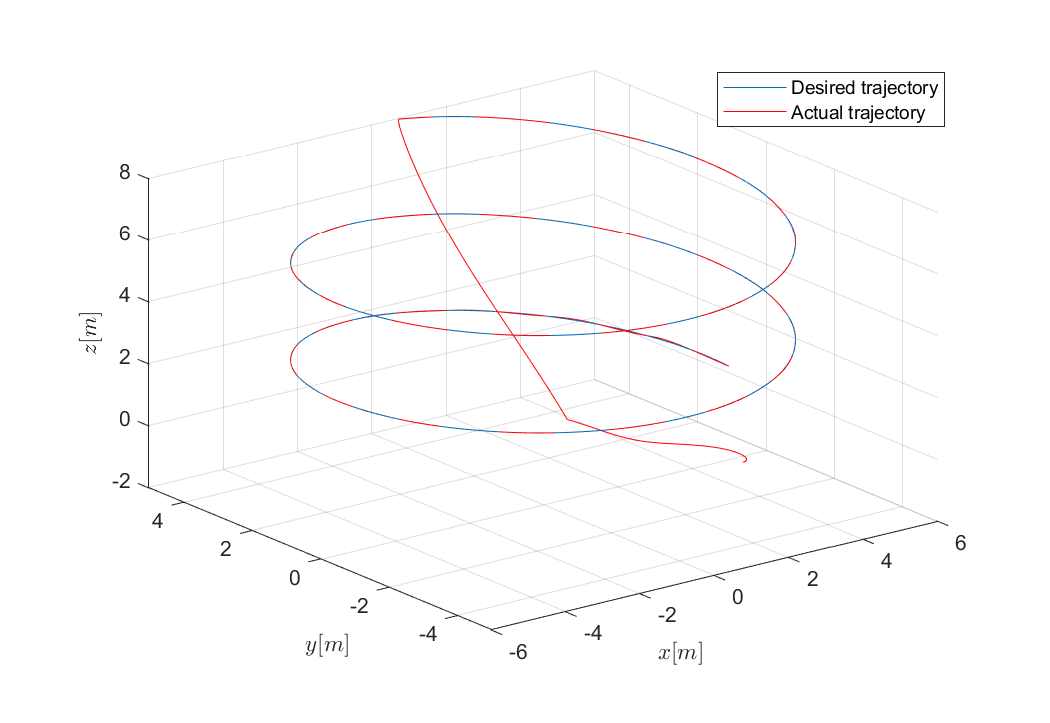
\includegraphics[scale=0.5]{figures/FL_trajectory}
    \caption{Trajectory tracking.}
    \label{fig:FL_trajectory}
\end{figure}
This phenomenon is also visible in Figure \ref{fig:FL_attitude}. Despite the pitch having, up to a certain point, an acceptable evolution, the roll exhibits noticeable fluctuations that induce Ingenuity to assume an unrealistic behavior. As an additional consequence, the small angles assumption of the previous signals is violated, leading to a significant error in the yaw angle, whose reference is not followed. Moreover, as in the previous graph, the abrupt change in the reference causes the bursting of the examined states.
\begin{figure}[H]
    \centering
    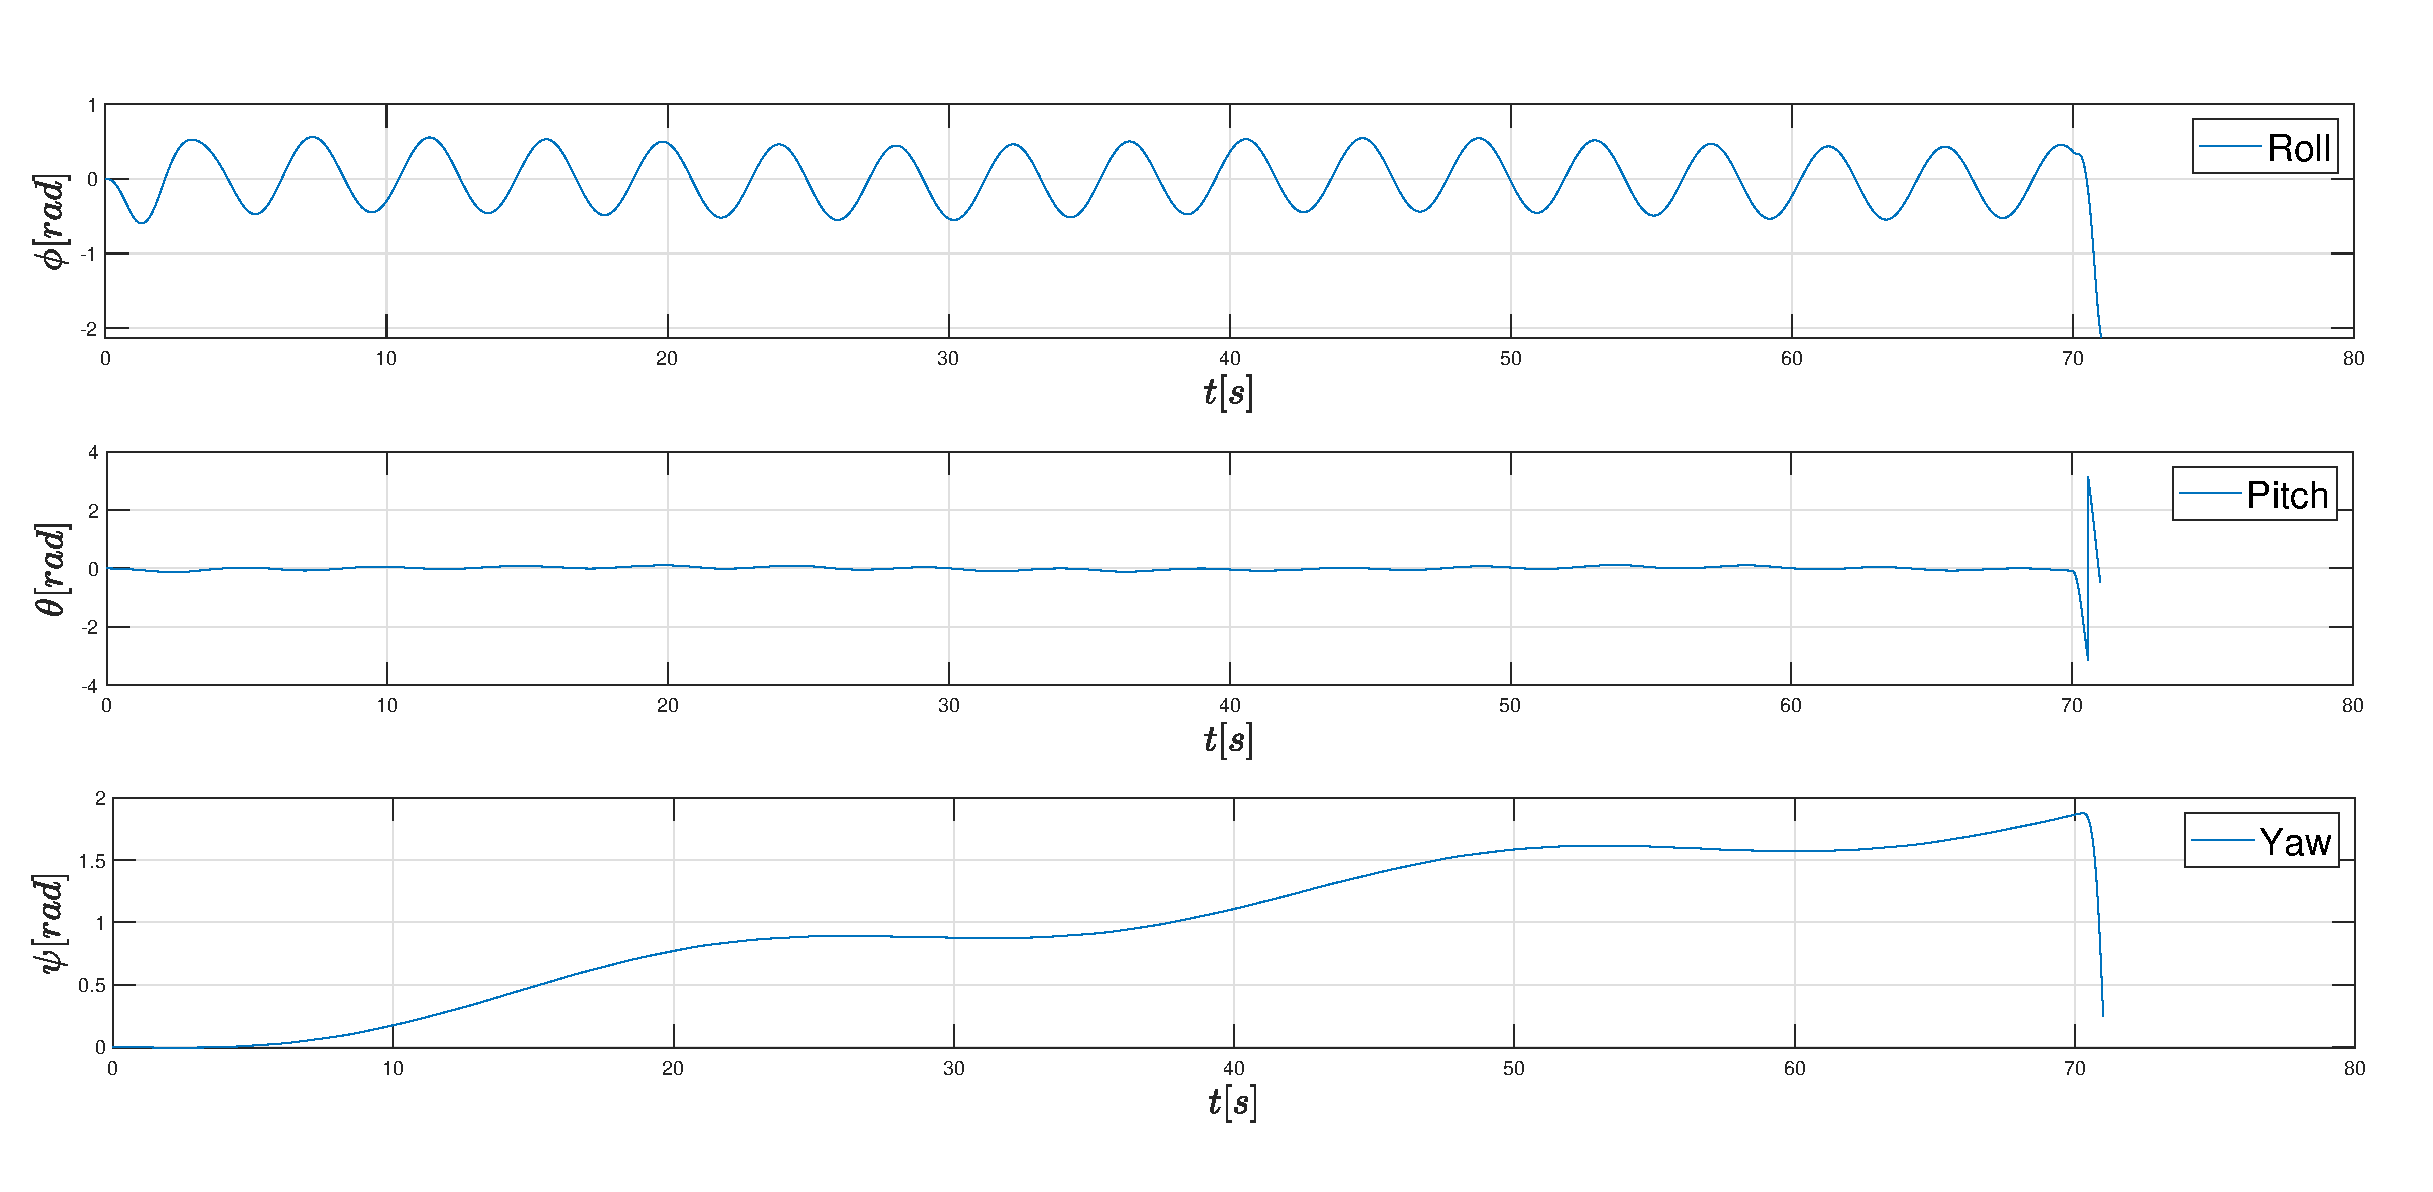
\includegraphics[scale=0.2]{figures/FL_attitude}
    \caption{Evolution of the roll, pitch and yaw angles respectively.}
    \label{fig:FL_attitude}
\end{figure}
The previous results can only be obtained if the inputs are not constrained. In fact, Figures \ref{fig:FL_angles} and \ref{fig:FL_omega} show that the value of the angle $\beta$ breaks the constraint \ref{eq:beta_constraint}. If saturations were imposed on the input signals, the system would fail to track the trajectory and diverge even in the initial phase.
\begin{figure}[H]
    \centering
    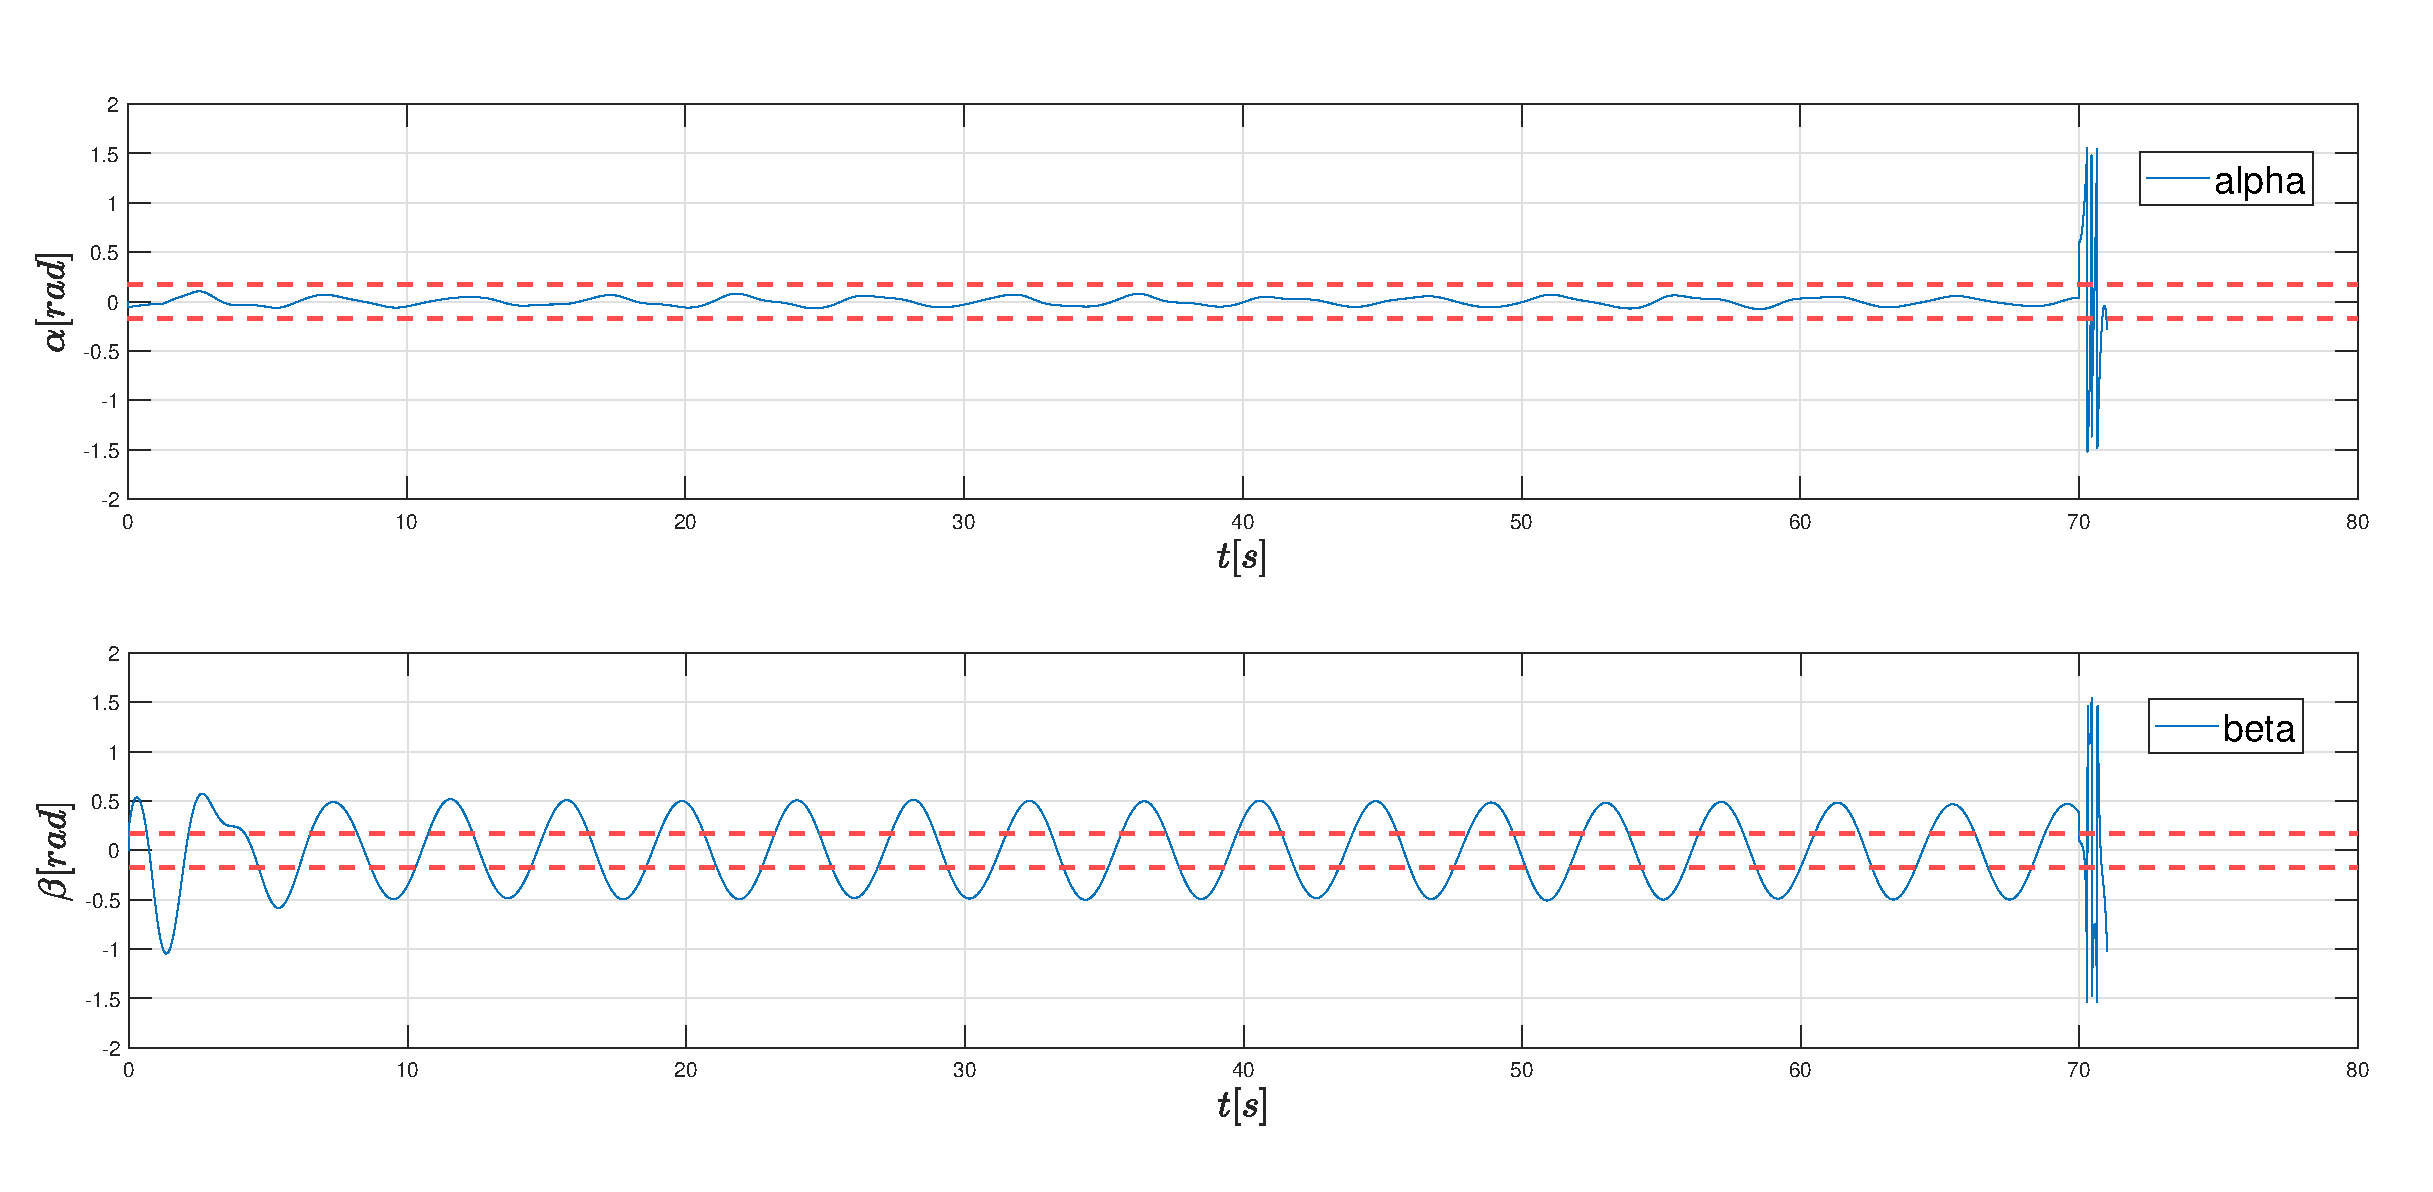
\includegraphics[scale=0.2]{figures/FL_angles}
    \caption{Angles $\alpha$ and $\beta$ of the swashplate.}
    \label{fig:FL_angles}
\end{figure}
\begin{figure}[H]
    \centering
    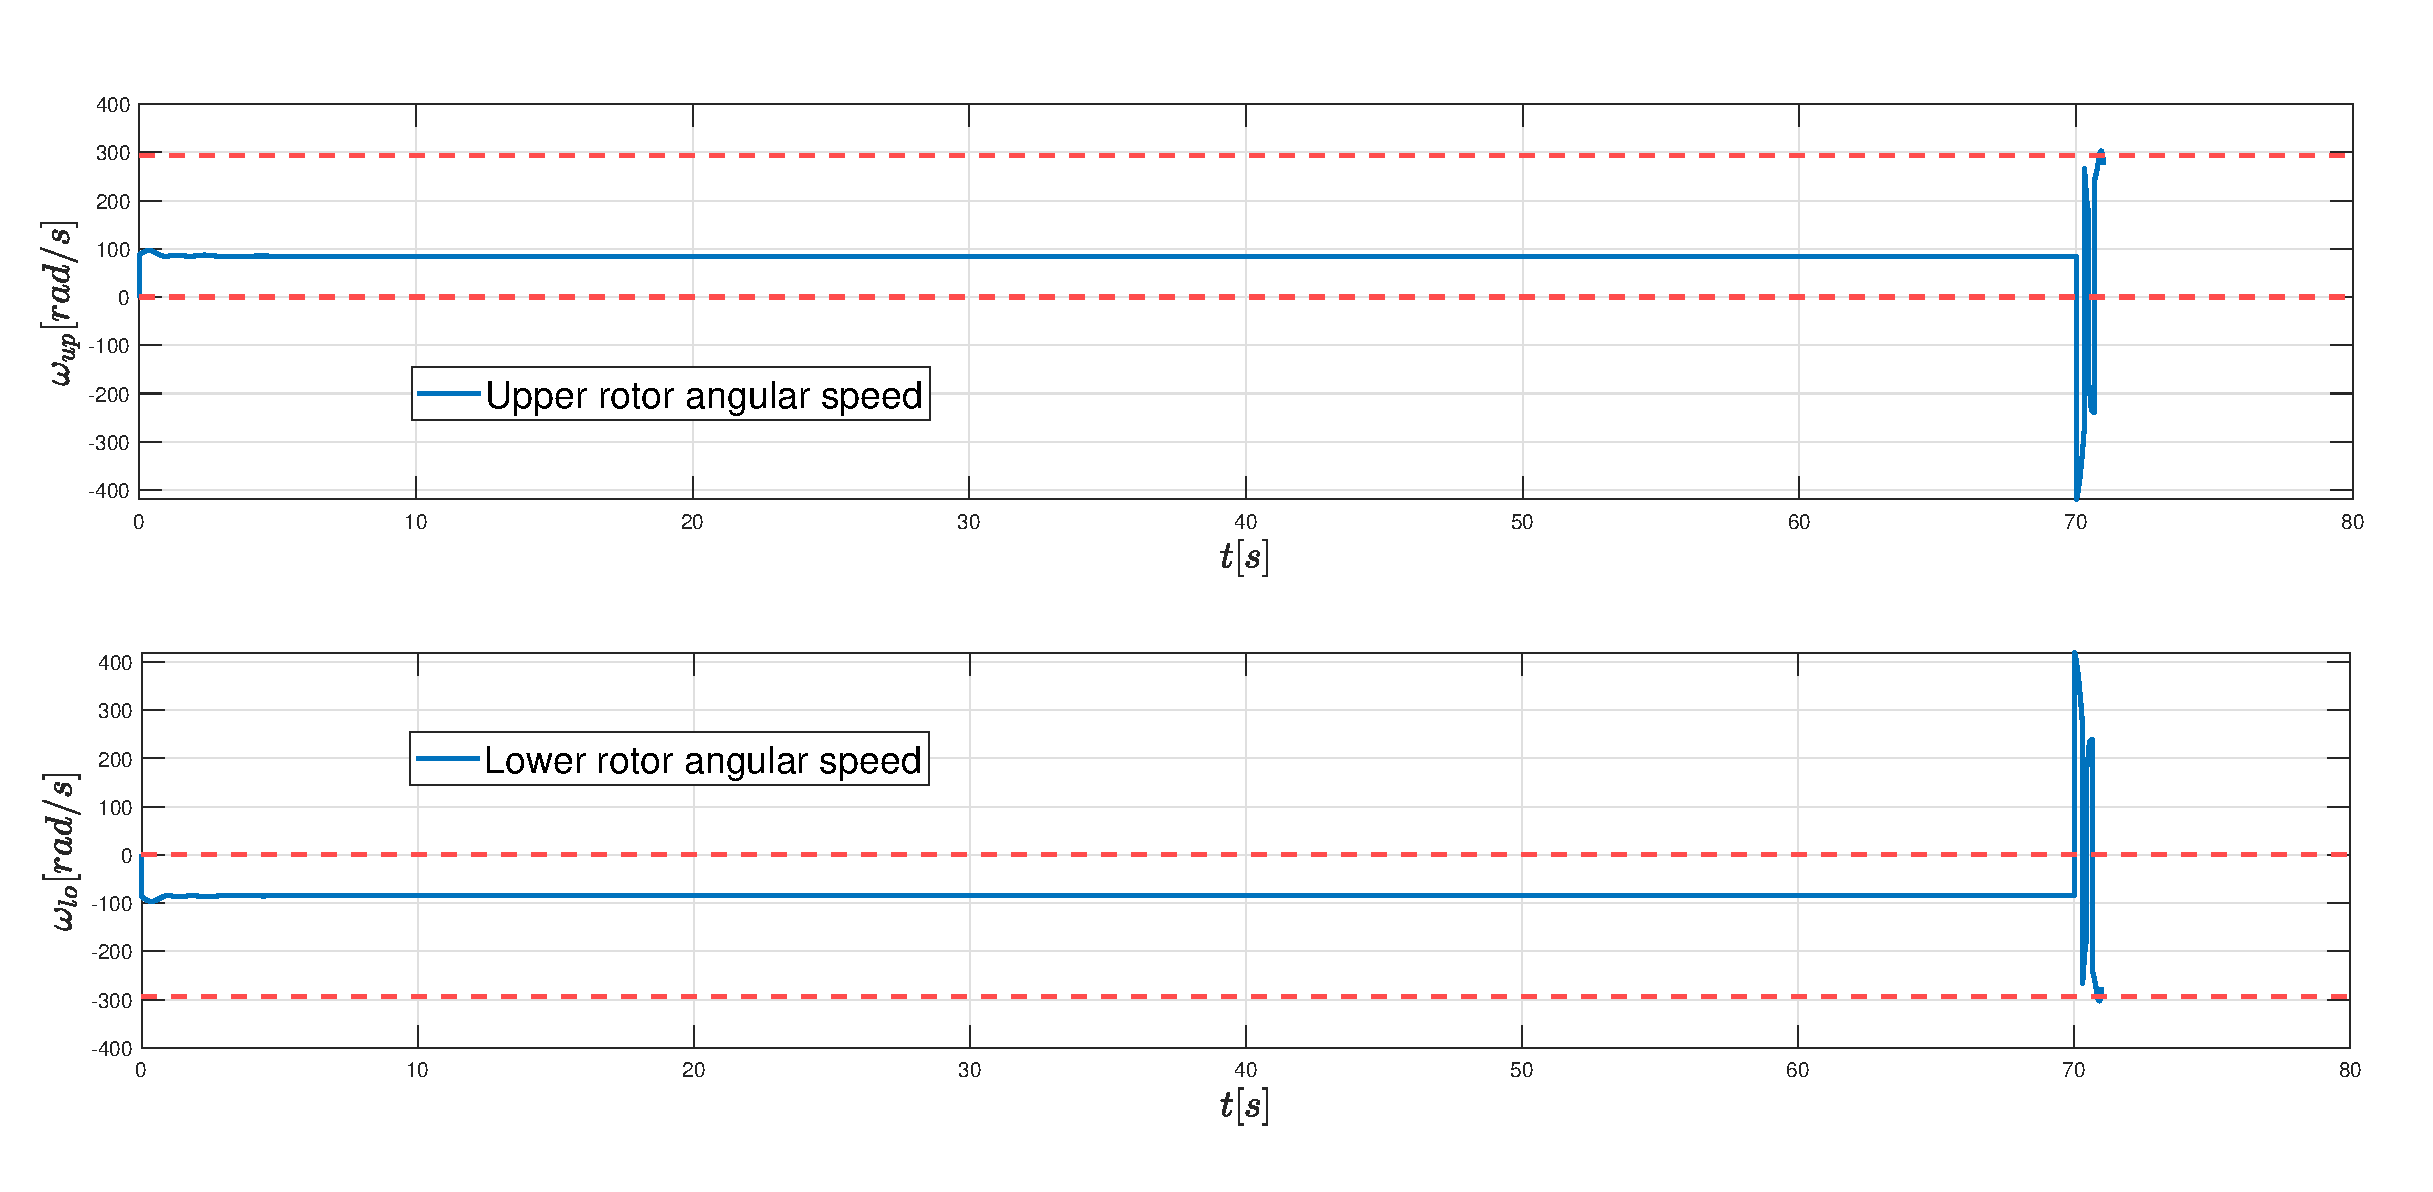
\includegraphics[scale=0.2]{figures/FL_omega}
    \caption{Angular velocities of the upper and lower rotor respectively.}
    \label{fig:FL_omega}
\end{figure}


    \section{Control via backstepping}\label{sec:backstepping}
In this section we will present the backstepping control technique applied to the helicopter model. The main idea is to act on the whole system to ultimately obtain global asymptotic stability and therefore track a desired trajectory.
Let us consider once again the state-space representation in \ref{eq:fbl_model}. In order to find an analytical solution to the control problem, we will assume that the horizontal components of the control input $u$ (defined in \ref{eq:u}) are negligible. This is justified by the fact that, in nominal operational conditions, the main contribution of the thrust generated by the rotors is the vertical one with respect to the body frame. Therefore $u$ can be written as: 
\begin{align}
    u=
    \begin{bmatrix} 
        0 \\ 0 \\ u_3
    \end{bmatrix}. \label{eq:u3}
\end{align}

The objective is to design a control law $(u, \tau_{tot}^b)$, depending only on the measurable states, such that the tracking error
\begin{align*}
    \varepsilon(t) \coloneq (P(t)-P^d(t),W_3(t)-W_3^d(t))
\end{align*}
is asymptotically stable for all initial conditions.

We start the procedure with the definition of the position error in the body reference frame:
\begin{align*}
    \delta_1 \coloneq R^T(P^d-P).
\end{align*}
Its time derivative is given by:
\begin{align*}
    \frac{d}{dt}\delta_1 &= -\Omega^b \times R^T(P^d-P) + R^T \left( \frac{d}{dt}P^d-\frac{d}{dt}P \right) \\
    &= -\Omega^b \times \delta_1+R^T \left( \frac{d}{dt}P^d-V^b \right).
\end{align*}
From this, we identify the velocity error in the body reference frame:
\begin{align*}
    \delta_2 \coloneq R^T \left( \frac{d}{dt}P^d-V^b \right).
\end{align*}
After differentiation with respect to time, we obtain:
\begin{align*}
    \frac{d}{dt}\delta_2 &= -\Omega^b \times \delta_2+R^T \frac{d^2}{dt^2}P^d-\frac{1}{m}(R^T F_g^i -u).
\end{align*}

Define as $V_1$ the first Lyapunov function, regarding the pseudo-energy of the position and velocity errors, as:
\begin{align*}
    V_1 \coloneq \frac{1}{2}(\delta_1+\lambda \delta_2)^T(\delta_1+\lambda \delta_2)+\frac{1}{2}\delta_1^T\delta_1,
\end{align*}
where $\lambda>0$ is a slack variable to be tuned. The time derivative of $V_1$ is:
\begin{align*}
    \frac{d}{dt}V_1 = (\delta_1+\lambda \delta_2)^T \left( \delta_2+\lambda R^T \frac{d^2}{dt^2}P^d-\frac{\lambda}{m}u \right)+\delta_1^T \delta_2.
\end{align*} \\
We are looking for a virtual control input $(\frac{\lambda}{m}u)^*$ making $\frac{d}{dt}V_1 \leq -V_1$ barring an error that has to be recovered in the next iteration of the backstepping procedure. The aforementioned virtual control is:
\begin{align*}
    \left( \frac{\lambda}{m}u \right)^* = \delta_1+\lambda \delta_2+2\delta_2+\lambda R^T \frac{d^2}{dt^2}P^d.
\end{align*}
This choice results in:
\begin{gather*}
    \frac{d}{dt}V_1 = -(\delta_1+\lambda \delta_2)^T(\delta_1+\lambda \delta_2)-\lambda \delta_2^T \delta_2 + \\
    (\delta_1+\lambda \delta_2)^T \delta_3,
\end{gather*}
where:
\begin{align*}
    \delta_3 \coloneq \left( \frac{\lambda}{m}u \right)^*-\frac{\lambda}{m}u.
\end{align*}

We proceed further by computing the time derivative of $\delta_3$ as:
\begin{gather*}
    \frac{d}{dt}\delta_3 = -\Omega^b \times \delta_3 -\frac{\lambda}{m}\Omega^b \times u+\frac{\lambda+2}{\lambda}\delta_3-\frac{\lambda+2}{\lambda}\delta_1 \\
    -\frac{(\lambda+2)^2-\lambda}{\lambda}\delta_2+\lambda R^T \frac{d^3}{dt^3}P^d-\frac{\lambda}{m}\frac{d}{dt}u.
\end{gather*}
Let us consider at this stage the error in the yaw component:
\begin{align*}
    \varepsilon_2 = W_3^d-W_3.
\end{align*}
The second Lyapunov function is:
\begin{align*}
    V_2 = \frac{1}{2}\delta_3^T\delta_3+\frac{1}{2}\varepsilon_2^2,
\end{align*}
with its time derivative being:
\begin{gather*}
    \frac{d}{dt}V_2 = \delta_3^T \bigg( -\Omega^b \times \delta_3-\frac{\lambda}{m}\Omega^b \times u - \frac{\lambda+2}{\lambda}\delta_1 + \\
    \frac{\lambda+2}{\lambda}\delta_3 - \frac{(\lambda +2)^2 - \lambda}{\lambda} \delta_2 + \lambda R^T \frac{d^3}{dt^3}P^d - \frac{\lambda}{m} \frac{d}{dt} u \bigg) \\
    + \varepsilon_2 \left( \frac{d}{dt}{W_3^d}-\frac{d}{dt}W_3 \right).
\end{gather*}

The third component\footnote{Notice that $\delta_3^T  (-\Omega^b \times \delta_3) = 0$ and $\Omega^b \times u = \begin{bmatrix}
    \star & \star & 0
\end{bmatrix}^T.$} of the first bracket in the previous equation can be directly shaped by imposing the value of the derivative of the lift $u$:
\begin{gather*}
    \frac{d}{dt}u_3 =  \frac{m}{\lambda} \begin{bmatrix}
        0 & 0 & 1 \end{bmatrix} \bigg( \frac{\lambda+2}{\lambda}\delta_3-\frac{\lambda+2}{\lambda}\delta_1 \\ -\frac{\lambda^2+3\lambda+4}{\lambda}\delta_2+\lambda R^T \frac{d^3}{dt^3}P^d+ \delta_1+\lambda \delta_2 \bigg).
\end{gather*}
The vector $\begin{bmatrix}
    0 & 0 & 1
\end{bmatrix}$ has been used to isolate the third component of the equation. The residual positional error is taken into account with the goal of imposing the decrease rate of $\frac{d}{dt} (V_1 + V_2)$ along the system trajectories with the choice of the virtual control:
\begin{gather*}
    \left( \frac{\lambda}{m} \Omega^b \times u \right)^* \coloneq \begin{bmatrix}
        1 & 0 & 0 \\ 0 & 1 & 0 \\ 0 & 0 & 0
    \end{bmatrix} \bigg( \frac{\lambda+2}{\lambda}\delta_3-\frac{\lambda+2}{\lambda}\delta_1 \\ -\frac{\lambda^2+3\lambda+4}{\lambda}\delta_2+\lambda R^T \frac{d^3}{dt^3}P^d+ \delta_1+\lambda \delta_2 + k_1 \delta_3 \bigg).
\end{gather*}
that lives in the orthogonal plane to $u_3$, where $k_1>0$ is slack variable to be tuned in order to determine the rate of convergence of the error $\delta_3$.\\
Through the last two choices, we have only controlled the part of $\frac{d}{dt}V_2$ regarding the position error.
Now we can focus on the yaw term by introducing the virtual control:
\begin{gather*}
    \left( \frac{d}{dt}W_3 \right)^* \coloneq \frac{d}{dt}W_3^d + k_2 \varepsilon_2,
\end{gather*}
The derivative of the second Lyapunov function becomes:
\begin{gather*}
    \frac{d}{dt}V_2 = \delta_3^T \delta_4-k_1 \delta_3^T \delta_3 - \delta_3^T (\delta_1+\lambda \delta_2)  - k_2 \varepsilon_2^2 + \varepsilon_2 \varepsilon_3,
\end{gather*}
where:
\begin{gather*}
    \delta_4 \coloneq \left( \frac{\lambda}{m} \Omega^b \times u \right)^* - \frac{\lambda}{m} \Omega^b \times u, \\
    \varepsilon_3 \coloneq \frac{d}{dt}W_3^* - \frac{d}{dt}W_3.
\end{gather*}

Finally, the last iteration starts with the computation of the time derivative of the latter:
\begin{gather*}
    \frac{d}{dt}\delta_4 = \frac{d}{dt} \left( \frac{\lambda}{m} \Omega^b \times u \right)^* - \frac{\lambda}{m} \left( \frac{d}{dt} \Omega^b \right) \times u  \\ - \frac{\lambda}{m} \Omega^b \times \left( \frac{d}{dt} u \right), \\
    \frac{d}{dt} \varepsilon_3 = \frac{d^2}{dt^2} W_3^d + k_2 \bigg(\frac{d}{dt} W_3^d - \frac{d}{dt} W_3 \bigg) - \frac{d^2}{dt^2} W_3.
\end{gather*}
At this point, we can define the third Lyapunov function and proceed as usual.
\begin{gather*}
    V_3 = \frac{1}{2} \delta_4^T \delta_4 + \frac{1}{2} \varepsilon_3^2.
\end{gather*}
Which, after differentiation, results in:
\begin{gather*}
    \frac{d}{dt}V_3 = \delta_4^T \bigg( \frac{d}{dt} \left( \frac{\lambda}{m} \Omega^b \times u \right)^* - \frac{\lambda}{m} \left( \frac{d}{dt} \Omega^b \right) \times u \\ - \frac{\lambda}{m} \Omega^b \times \left( \frac{d}{dt} u \right) \bigg) \\
    + \varepsilon_3 \bigg( \frac{d^2}{dt^2} W_3^d + k_2 \bigg( \frac{d}{dt} W_3^d - \frac{d}{dt} W_3 \bigg) - \frac{d^2}{dt^2} W_3 \bigg).
\end{gather*}
Once again, our  goal is to "stabilize" the function $\frac{d}{dt}V_3$. This can be achieved through the following choices:
\begin{align*}
	\frac{d^2}{dt^2} W_3 = \frac{d^2}{dt^2} W_3^d + k_2\bigg( \frac{d}{dt} W_3^d - \frac{d}{dt} W_3 \bigg) + k_4\varepsilon_3 + \varepsilon_2,
\end{align*}
\begin{gather*}
	 \frac{\lambda}{m} \left( \frac{d}{dt} \Omega^b \right) \times u =  \frac{d}{dt} \left( \frac{\lambda}{m} \Omega^b \times u \right)^* - \frac{\lambda}{m} \Omega^b \times \left(\frac{d}{dt} u\right) \\ + \begin{bmatrix} 1 & 0 & 0 \\ 0 & 1 & 0 \\ 0 & 0 & 0 \end{bmatrix}\delta_3 + k_3\delta_4.
\end{gather*}
The very last equation results into the following expressions for the derivatives of the angular velocities in the body frame:
\begin{gather*}
	\frac{d}{dt} \Omega^b_1 = -\frac{m}{\lambda u_3}\begin{bmatrix}0 & 1 & 0\end{bmatrix}\bigg[ \frac{d}{dt} \left( \frac{\lambda}{m} \Omega^b \times u \right)^* -\\ \frac{\lambda}{m} \Omega^b \times \left(\frac{d}{dt} u\right) + \delta_3 + k_3\delta_4 \bigg], \\
	\frac{d}{dt} \Omega^b_2 = \frac{m}{\lambda u_3}\begin{bmatrix}1 & 0 & 0\end{bmatrix}\bigg[ \frac{d}{dt} \left( \frac{\lambda}{m} \Omega^b \times u \right)^* -\\ \frac{\lambda}{m} \Omega^b \times \left(\frac{d}{dt} u\right) + \delta_3 + k_3\delta_4 \bigg].
\end{gather*}
According to the above choices, the derivative of the third Lyapunov function becomes:
\begin{align*}
	\frac{d}{dt}V_3 = -k_4\varepsilon^2_3 - \varepsilon_2\varepsilon_3 - \delta_4^T\delta_3 - k_3\delta_4^T\delta_4.
\end{align*}

To summarize, consider the sum of the three aforementioned Lyapunov functions as the overall Lyapunov function $V$:
\begin{gather*}
	V=V_1+V_2+V_3=\frac{1}{2}(\delta_1+\lambda\delta_2)^T(\delta_1+\lambda\delta_2)+\\\frac{1}{2}\delta_1^T\delta_1+\frac{1}{2}\delta_3^T\delta_3+\frac{1}{2}\epsilon_2^2+\frac{1}{2}\delta_4^T\delta_4+\frac{1}{2}\epsilon_3^2,
\end{gather*}
with its time derivative being:
\begin{gather*}
	\frac{d}{dt}V=-(\delta_1+\lambda\delta_2)^T(\delta_1+\lambda\delta_2)-\lambda\delta_2^T\delta_2-k_1\delta_3^T\delta_3\\-k_2\varepsilon_2^2-k_4\varepsilon_3^2-k_3\delta_4^T\delta_4,
\end{gather*}
meaning that $V$ is monotonically decreasing (and thus the control objective is achieved) if and only if we pick the following:
\begin{gather*}
    \frac{d}{dt}u_3 =  \frac{m}{\lambda} \begin{bmatrix}
        0 & 0 & 1 \end{bmatrix} \bigg( \frac{\lambda+2}{\lambda}\delta_3-\frac{\lambda+2}{\lambda}\delta_1 \\ -\frac{\lambda^2+3\lambda+4}{\lambda}\delta_2+\lambda R^T \frac{d^3}{dt^3}P^d+ \delta_1+\lambda \delta_2 \bigg), \\
        \frac{d}{dt} \Omega^b_1 = -\frac{m}{\lambda u_3}\begin{bmatrix}0 & 1 & 0\end{bmatrix}\bigg[ \frac{d}{dt} \left( \frac{\lambda}{m} \Omega^b \times u \right)^* -\\ \frac{\lambda}{m} \Omega^b \times \left(\frac{d}{dt} u\right) + \delta_3 + k_3\delta_4 \bigg], \\
        \frac{d}{dt} \Omega^b_2 = \frac{m}{\lambda u_3}\begin{bmatrix}1 & 0 & 0\end{bmatrix}\bigg[ \frac{d}{dt} \left( \frac{\lambda}{m} \Omega^b \times u \right)^* -\\ \frac{\lambda}{m} \Omega^b \times \left(\frac{d}{dt} u\right) + \delta_3 + k_3\delta_4 \bigg], \\
        \frac{d}{dt} \Omega^b_3 = \frac{c_2}{c_1} \bigg( \frac{d^2}{dt^2} W_3^d + k_2\bigg( \frac{d}{dt} W_3^d - \frac{d}{dt} W_3 \bigg) + k_4\varepsilon_3 \\
        + \varepsilon_2 + \begin{bmatrix} 0 & 0 & 1 \end{bmatrix} M^{-1} \frac{d}{dt} M \, M^{-1} \Omega^b- \frac{s_1}{c_2} \frac{d}{dt} \Omega^b_2 \bigg).
\end{gather*}
with the latter resulting from the differentiation of the yaw angle $W_3$, and $M$ being:
\begin{align*}
    M = \begin{bmatrix}
        -s_2 & 0 & 1 \\ c_2s_1 & c_1 & 0 \\ c_2c_1 & -s_1 & 0
    \end{bmatrix}.
\end{align*}

\subsection{Actuation}
This section is the analogue of Section \ref{sec:fbl_actuation} for the backstepping controller. 
\\The backstepping procedure yields the values of the time derivative of the lift $\frac{d}{dt} u$ and the desired angular velocity dynamics $\frac{d}{dt}\Omega^b$, which must be converted into the actual inputs of the robot $\omega_u$, $\omega_l$, $\alpha$, and $\beta$.

For simplicity, let us use the following notation:
\begin{align*}
    \tau \coloneq \tau_{tot}^b.
\end{align*}
Assuming that $\alpha$ and $\beta$ are small:
\begin{align*}
    T_{(\alpha,\beta)}\approx \begin{bmatrix}
        \alpha\\\beta\\1
    \end{bmatrix},
\end{align*}
by \ref{eq:force_norm}, \ref{eq:force}, \ref{eq:torque_due_force}, \ref{eq:reaction_torque} and \ref{eq:torque}, we obtain a system of four equations in four unknowns:
\begin{equation*}
    \left\{\begin{array}{@{}l@{}}
\begin{bmatrix}
    \tau_1\\\tau_2\\\tau_3\\
\end{bmatrix}=\begin{bmatrix}
    -\beta \, (K_l-K_d) \, (d_{cm,u} \, \omega_u^2+d_{cm,l} \, \omega_l^2)\\
    \alpha \, (K_l-K_d) \, (d_{cm,u} \, \omega_u^2+d_{cm,l} \, \omega_l^2)\\
    0.02 \, (K_l-K_d) \, (\omega_u^2-\omega_l^2)
\end{bmatrix} \\
u_3=(K_l-K_d)(\omega_u^2+\omega_l^2)

\end{array}\right. ,
     \end{equation*}
whose (real) solutions exist only if the following condition is satisfied:
$$|\tau_3| \leq \frac{u_3}{50}.$$
In that case, the solutions are:
\begin{gather*}
    w_u=\sqrt{\frac{u_3+50 \, \tau_3}{2(K_l-K_d)}}\\
    w_l=\sqrt{\frac{u_3-50 \, \tau_3}{2(K_l-K_d)}}\\
    \alpha=\frac{2\tau_2}{(d_{cm,l}+d_{cm,u}) \, u_3+50 \, (d_{cm,u}-d_{cm,l}) \, \tau_3}\\
    \beta=\frac{-2\tau_1}{(d_{cm,l}+d_{cm,u}) \, u_3+50 \, (d_{cm,u}-d_{cm,l}) \, \tau_3},
\end{gather*}
where $\tau_1$, $\tau_2$ and $\tau_3$ are the three components of $\tau$, whose value comes from \ref{eq:fbl_model}:
\begin{align*}
    \tau=I\frac{d}{dt}\Omega^b + \Omega^b \times (I\Omega^b).
\end{align*}
\subsection{Simulation results} 
The backstepping controller was also tested on the a trajectory tracking task akin to the one seen in Section \ref{sec:fbl_sim}. The reference trajectory is expressed in \ref{eq:pos_ref} and \ref{eq:yaw_ref}, with the same parameters $r = \qty{5}{\meter}$, $d = 5$ and $k = 10$. 
\\With the current controller, which is far more robust than of the previous one, we can also afford to start from an initial condition corresponding to a nonzero initial tracking error, i.e., the origin.

The comparison between the reference and the actual trajectory of Ingenuity is shown in Figure \ref{fig:BS_trajectory}. Notice that the robot is able to follow the desired path with a good approximation, while recovering both the initial position error and the final one (generated by the abrupt change in the reference). 
\begin{figure}[H]
    \centering
    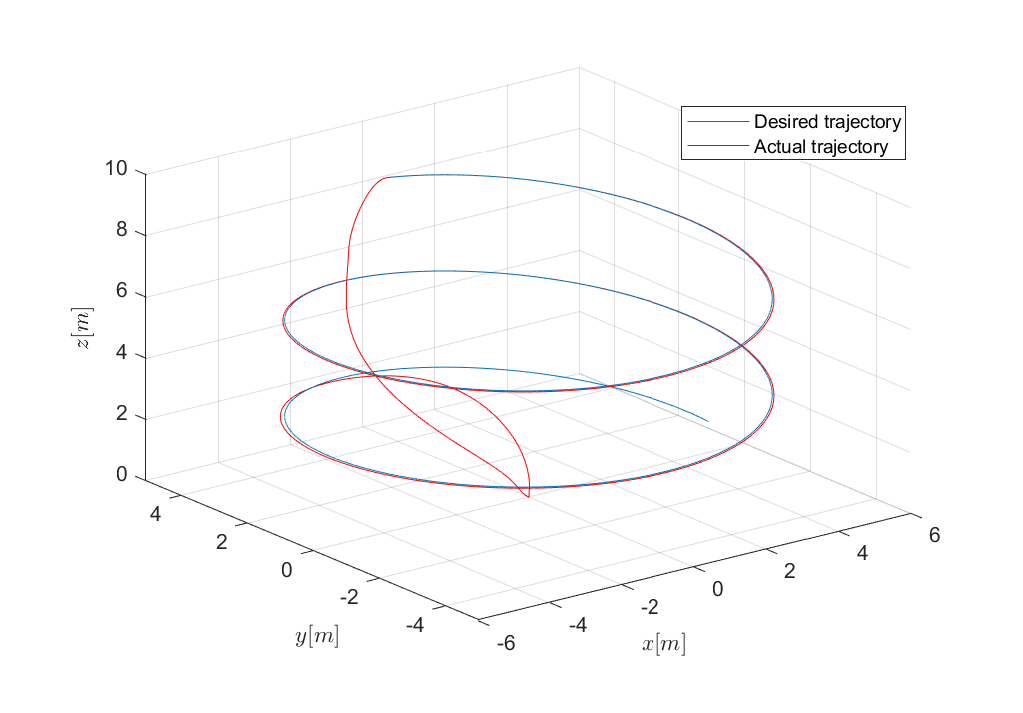
\includegraphics[scale=0.5]{figures/BS_trajectory}
    \caption{Trajectory tracking.}
    \label{fig:BS_trajectory}
\end{figure}
As theoretically expected, the controller exploits the roll and pitch dynamics to impart the desired behavior to the remainder of the system (see Figure \ref{fig:BS_attitude}). 
\begin{figure}[H]
    \centering
    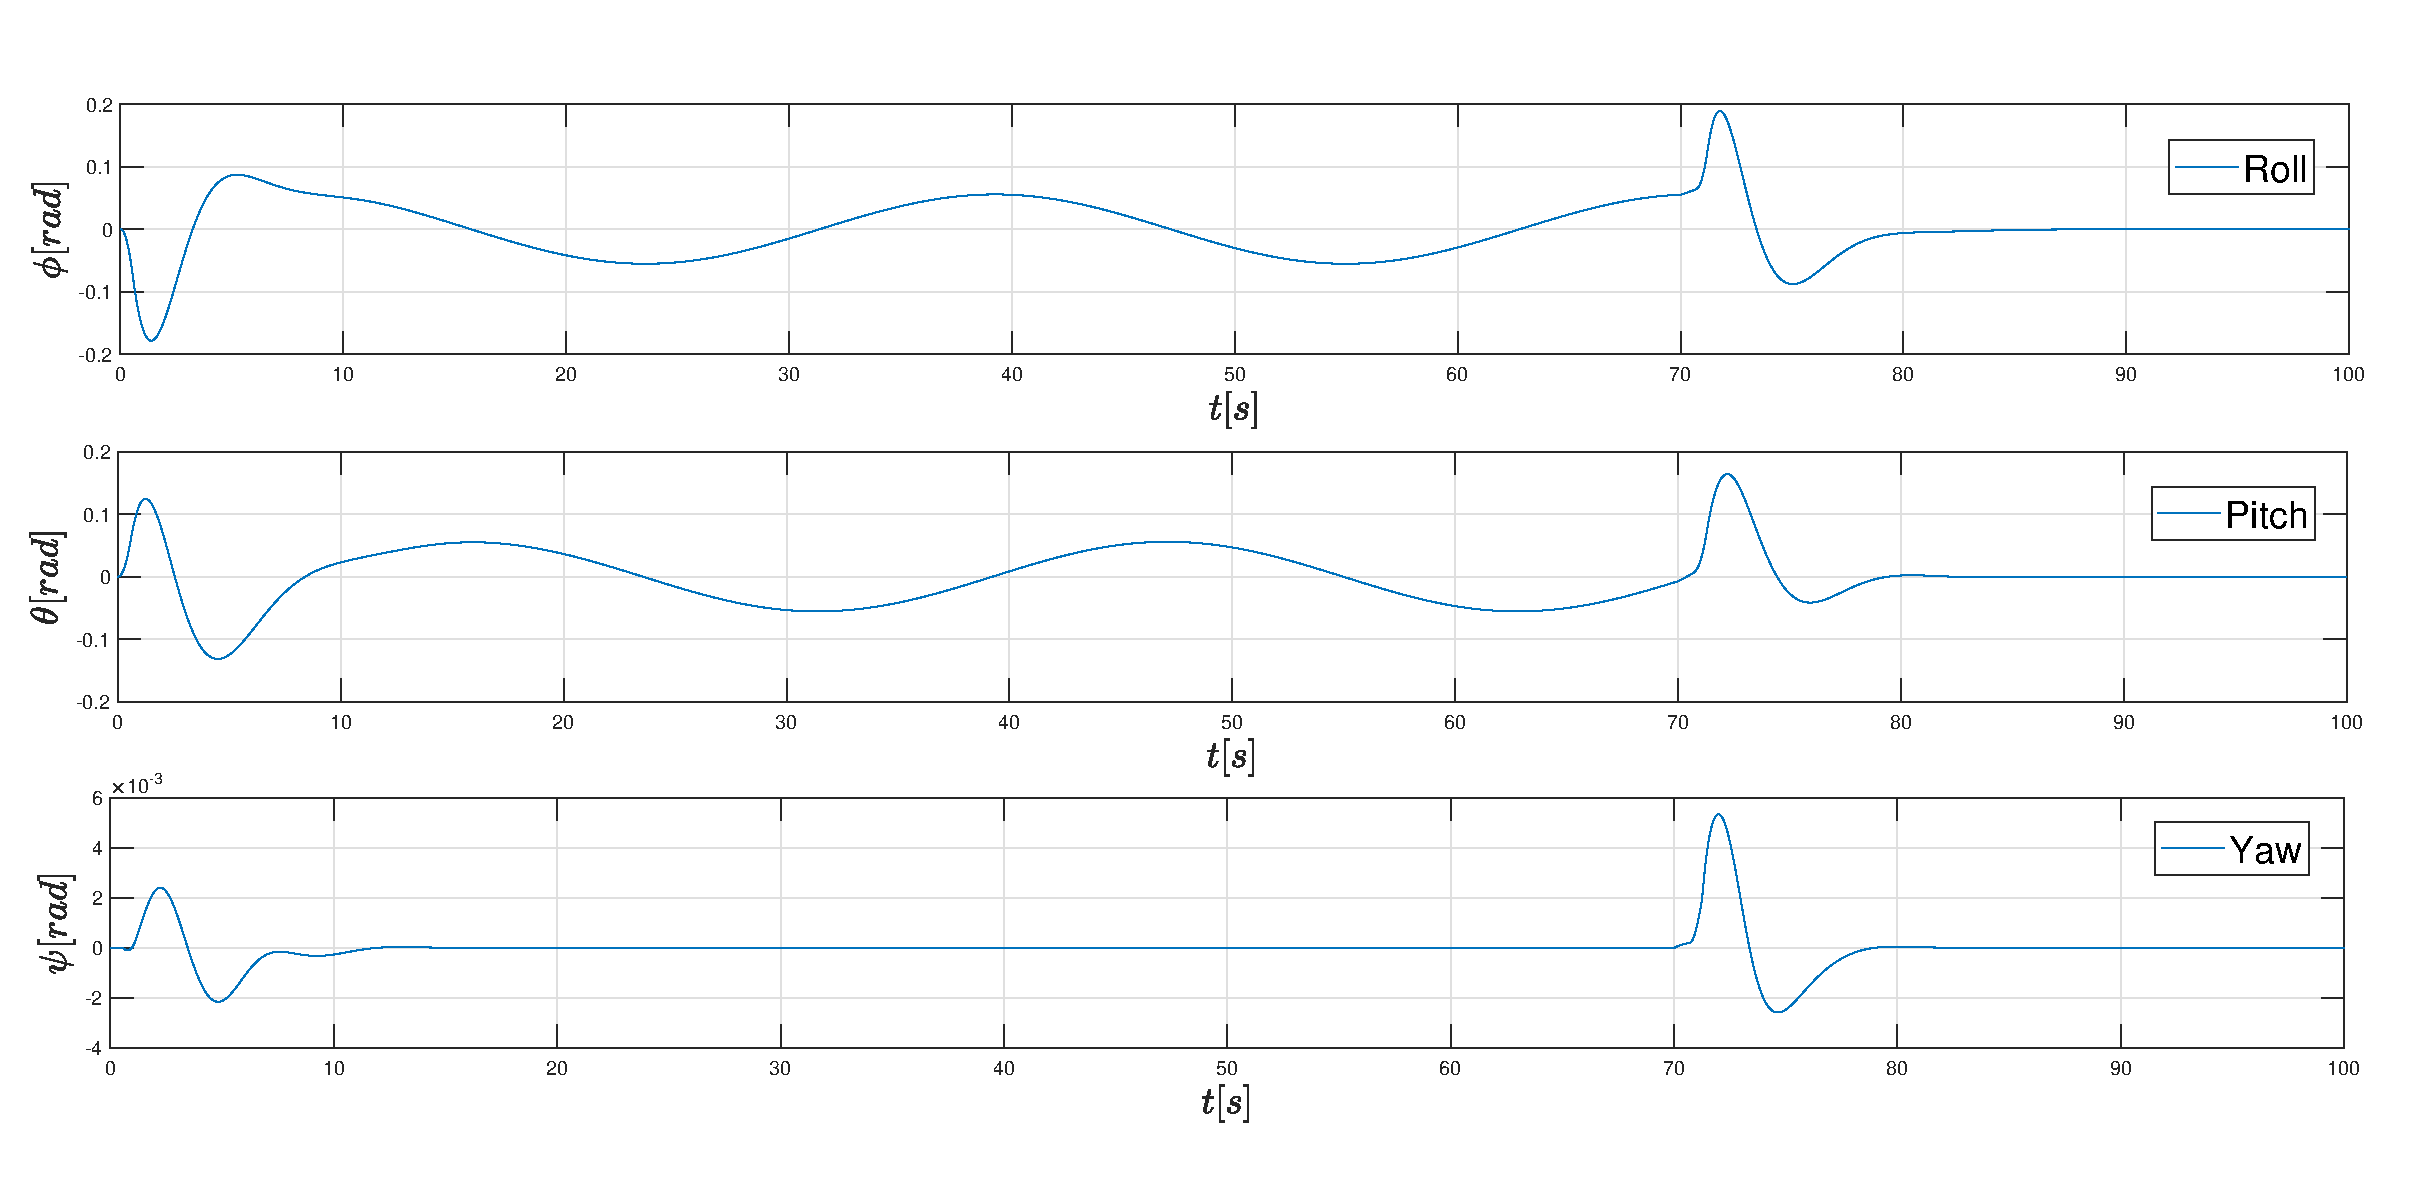
\includegraphics[scale=0.2]{figures/BS_attitude}
    \caption{Evolution of the roll, pitch and yaw angles respectively.}
    \label{fig:BS_attitude}
\end{figure}
Finally, the necessary control inputs, adequately saturated according to the constraints \ref{eq:omega_u_constraint} - \ref{eq:beta_constraint} so as to reflect the actual physical limitations of the actuators, are depicted in Figures \ref{fig:BS_angles} and \ref{fig:BS_omega}. 
\\ We can therefore state that the controller is not only robust to external disturbances, but also to these types of constraints.
\begin{figure}[H]
    \centering
    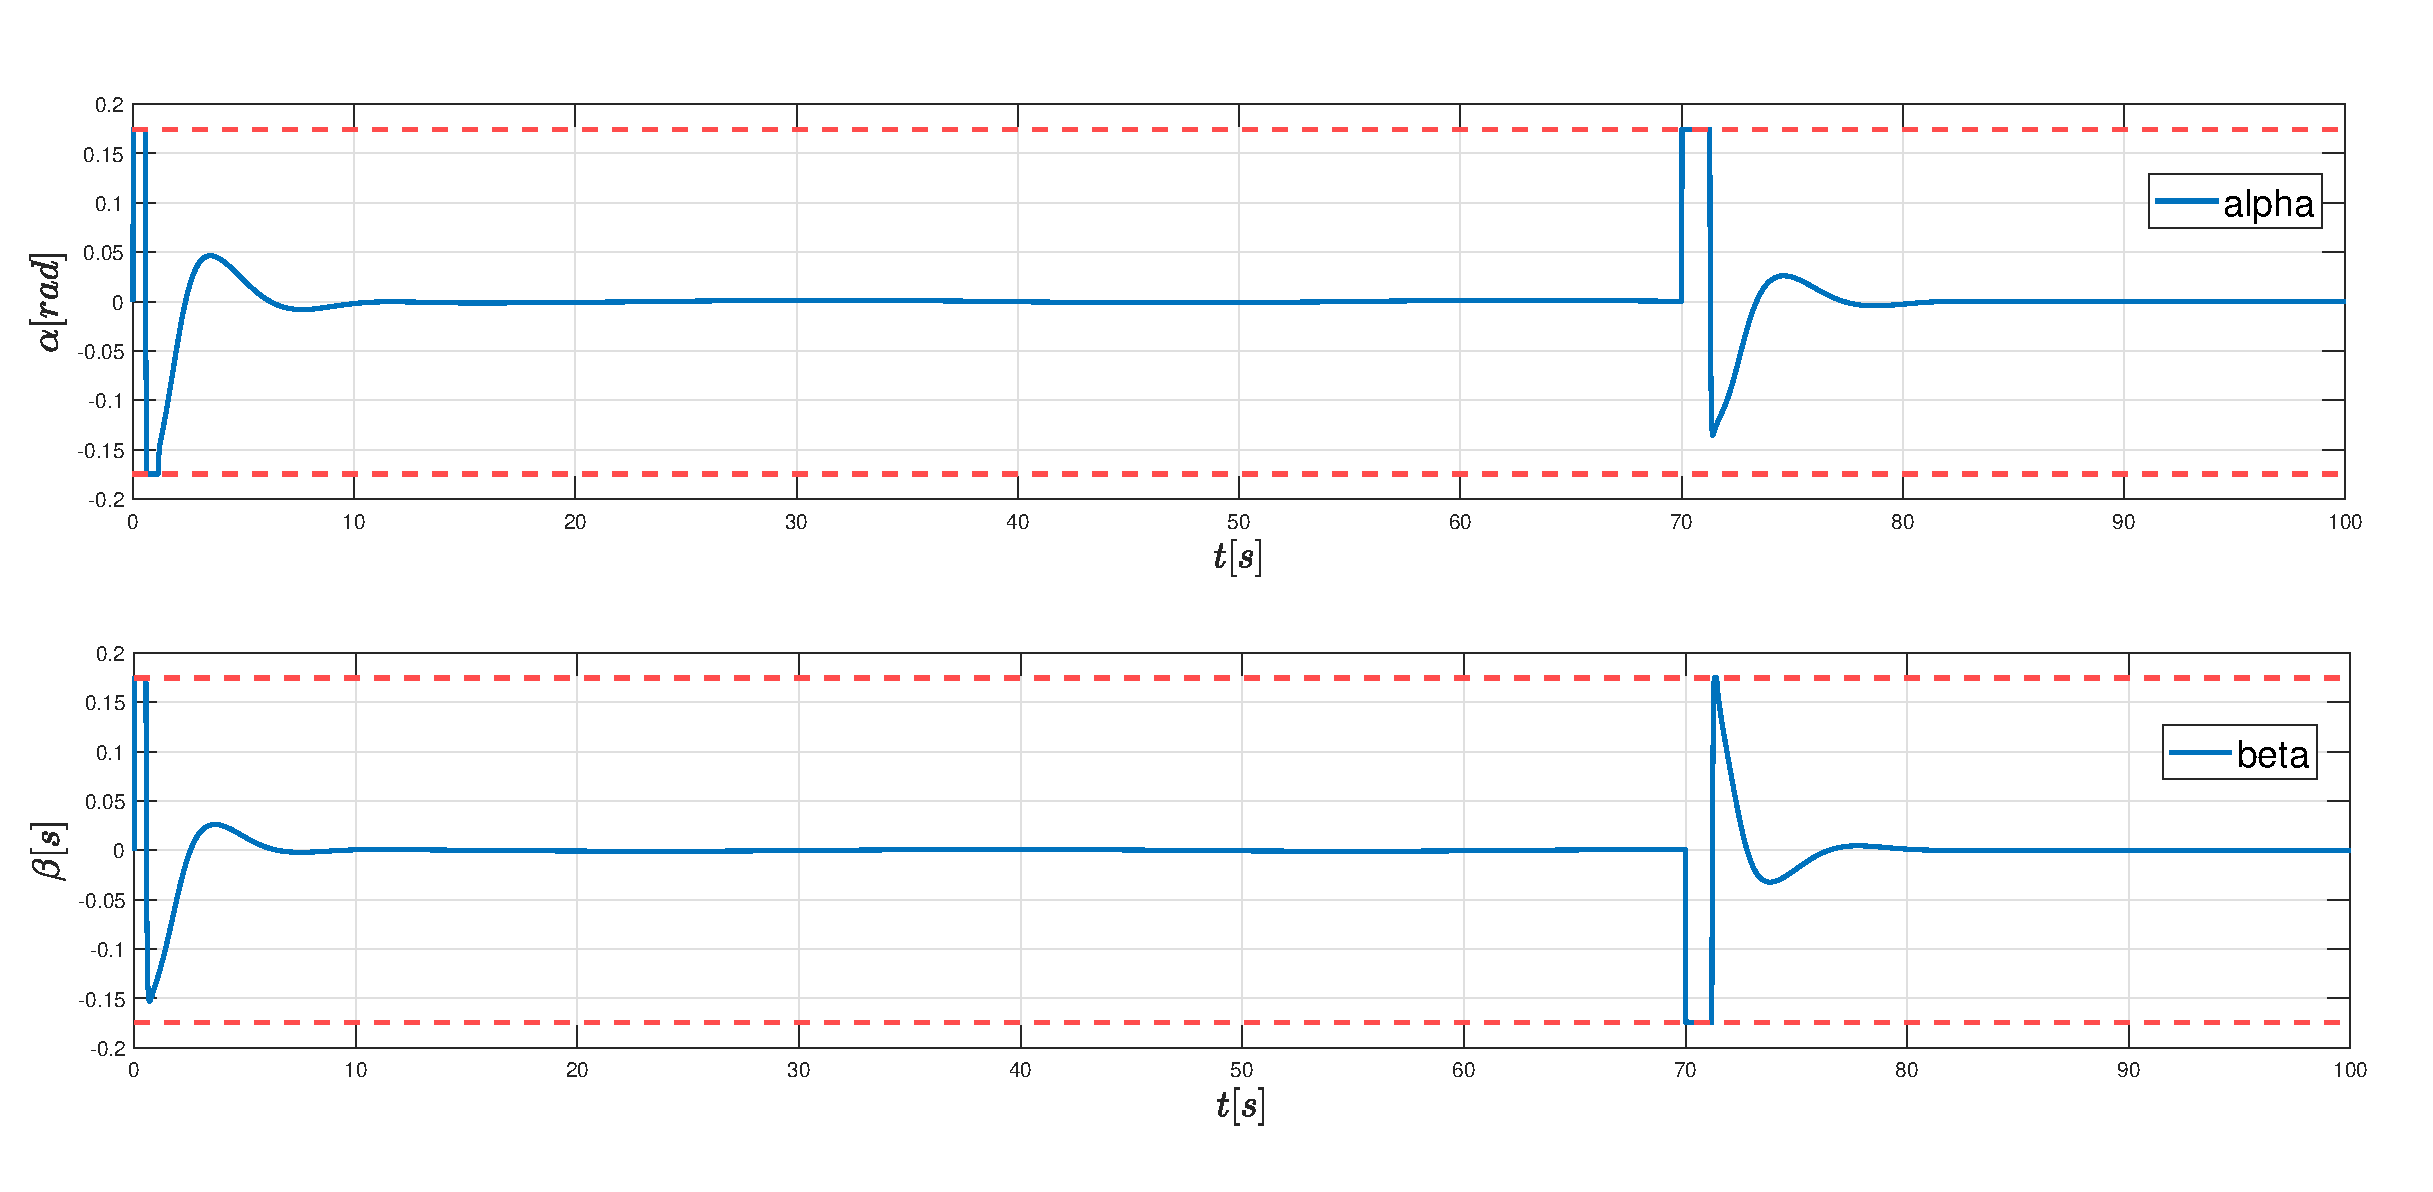
\includegraphics[scale=0.2]{figures/BS_angles}
    \caption{Angles $\alpha$ and $\beta$ of the swashplate.}
    \label{fig:BS_angles}
\end{figure}
\begin{figure}[H]
    \centering
    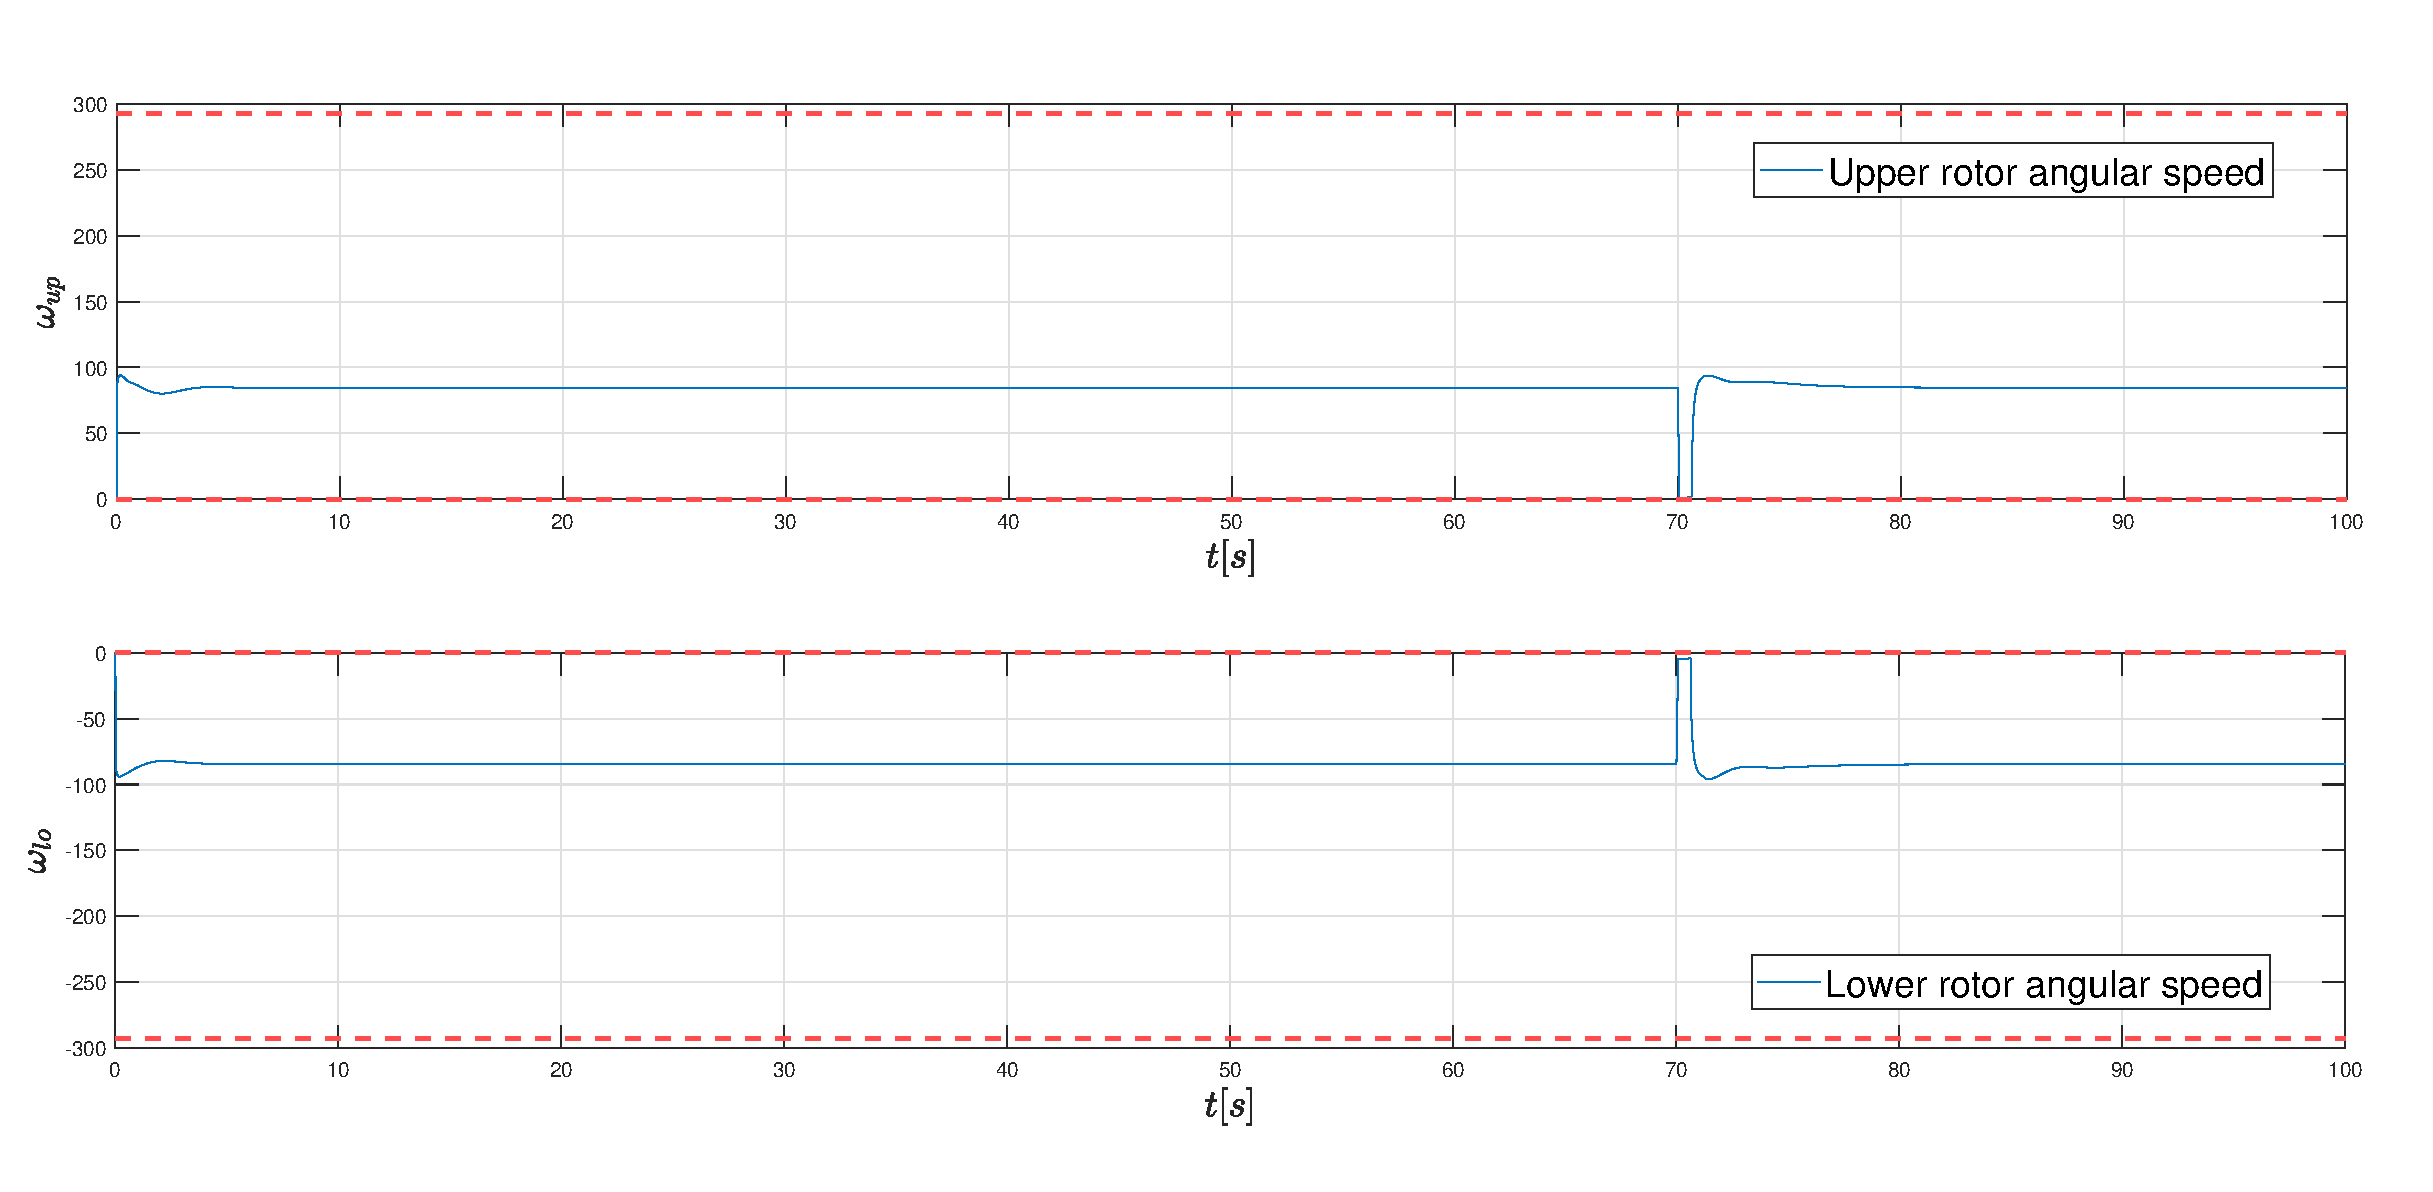
\includegraphics[scale=0.2]{figures/BS_omega}
    \caption{Angular velocities of the upper and lower rotor respectively.}
    \label{fig:BS_omega}
\end{figure}




% \[\frac{d}{dt}L=-(\delta_1+\lambda\delta_2)^T(\delta_1+\lambda\delta_2)-\lambda\delta_2^T\delta_2+(\delta_1+\lambda\delta_2)^T\delta_3+\]\[-K_1\delta_3^T\delta_3-\delta_3^T(\delta_1+\lambda\delta_2)+\delta_3^T\delta_4-K_2\epsilon_2^2+\epsilon_2\epsilon_3-K_4\epsilon_3^2-\epsilon_2\epsilon_3+\]\[-\delta_4^T\delta_3-K_3\delta_4^T\delta_4=
% -(\delta_1+\lambda\delta_2)^T(\delta_1+\lambda\delta_2)-\lambda\delta_2^T\delta_2-K_1\delta_3^T\delta_3+\]\[-K_2\epsilon_2^2-K_4\epsilon_3^2-K_3\delta_4^T\delta_4\]

% The time derivative is 
% \[
% \frac{d}{dt}V_1=(\delta_1+\lambda \delta_2)^T 
% \Bigg[-\Omega^b \times\delta_1+\delta_2+ \lambda\Bigg(-\Omega^b \times\delta_2+\]\[+R^T\ddot{P^d}-\frac{F}{m}\Bigg)\Bigg]+\delta_1^T\left(-\Omega \times \delta_1 +\delta_2\right)=\]\[=(\delta_1+\lambda \delta_2)^T\left(\delta_2+\lambda R^T\ddot{P^d}-\frac{\lambda F}{m}\right)+\delta_1^T\delta_2 \]
% The desired value of the actual force, considered as virtual input gives
% \[\left(\frac{\lambda}{m}F\right)^*=\delta_1+\lambda \delta_2+2\delta_2+\lambda R^T\ddot{P^d}\]
% From which we get 
% \[\frac{d}{dt}V_1=-(\delta_1+\lambda \delta_2)^T(\delta_1+\lambda \delta_2)-\lambda\delta_2^T\delta_2+\]\[+(\delta_1+\lambda \delta_2)^T\frac{\lambda}{m}(F^*-F)\]
% where the error between the virtual force
% and the actual force $\delta_3=(\frac{\lambda}{m}F)^*-\frac{\lambda}{m}F $ appears.\\
% Its derivative is 
% \[\frac{d}{dt}\delta_3=\frac{d}{dt}\left(\frac{\lambda}{m}F\right)^*-\frac{d}{dt}\left(\frac{\lambda}{m}F\right)=\]\[=
% \frac{d}{dt}(\delta_1+\lambda \delta_2+2\delta_2+\lambda R^T\ddot{P^d})-\frac{\lambda}{m}\frac{d}{dt}(R^TF_g^i+u)=\]\[=
% -\Omega^b \times \delta_1+\delta_2+(\lambda+2)\left(-\Omega^b \times \delta_2+R^T\ddot{P^d}-\frac{F}{m}\right)+\]\[+\lambda R^T\dddot{P^d}-\lambda\Omega^b \times R^T\ddot{P^d}+\frac{\lambda}{m}\Omega^b \times R^TF_g^i-\frac{\lambda}{m}\left(\frac{d}{dt}u\right)=\]\[=
% -\Omega^b \times \left(\delta_1+\lambda \delta_2+2\delta_2+\lambda R^T\ddot{P^d}-\frac{\lambda}{m} R^TF_g^i-\frac{\lambda}{m}u\right)\]\[-\frac{\lambda}{m}\Omega^b \times u+\delta_2+(\lambda+2)\left(R^T\ddot{P^d}-\frac{F}{m}\right)+\]\[+\lambda R^T\dddot{P^d}-\frac{\lambda}{m}\left(\frac{d}{dt}u\right)=
% -\Omega^b \times \delta_3 -\frac{\lambda}{m}\Omega^b \times u+\]\[+\frac{\lambda+2}{\lambda}\left(\lambda R^T\ddot{P^d}-\frac{\lambda}{m}F+\delta_1+\lambda \delta_2+2\lambda_2\right)+\]\[-\frac{\lambda+2}{\lambda}\left(\delta_1+\lambda \delta_2+2\lambda_2\right)+\delta_2+\lambda R^T\dddot{P^d}-\frac{\lambda}{m}\left(\frac{d}{dt}u\right)=\]\[=
% -\Omega^b \times \delta_3 -\frac{\lambda}{m}\Omega^b \times u+\frac{\lambda+2}{\lambda}\delta_3-\frac{\lambda+2}{\lambda}\delta_1-\frac{(\lambda+2)^2-\lambda}{\lambda}\delta_2+\]\[+\lambda R^T\dddot{P^d}-\frac{\lambda}{m}\left(\frac{d}{dt}u\right)
% \]
% Regarding the yaw control, we have the error
% \[\epsilon_2 := w_{3,d}-w_3\]
% and its derivative
% \[\frac{d}{dt}\epsilon_2=\dot{w_{3,d}}-\frac{d}{dt}w_3\]
% The second Lyapunov function is then
% \[V_2=\frac{1}{2}\delta_3^T\delta_3+\frac{1}{2}\epsilon_2^2\]
% Differentiating we get
% \[\frac{d}{dt}V_2=\delta_3^T\Bigg[-\Omega^b \times \delta_3-\frac{\lambda}{m}\Omega^b \times u+\frac{\lambda+2}{\lambda}\delta_3-\frac{\lambda+2}{\lambda}\delta_1+\]\[-\frac{(\lambda+2)^2-\lambda}{\lambda}\delta_2+\lambda R^T\dddot{P^d}-\frac{\lambda}{m}\left(\frac{d}{dt}u\right)\Bigg]+\epsilon_2\left(\dot{w_{3,d}}-\frac{d}{dt}w_3\right)\]
% Since $\frac{d}{dt}u$ and $\Omega$ are completely decoupled we can affect directly the input $\frac{d}{dt}u$. In particular we impose
% \[\frac{d}{dt}u_3=\frac{m}{\lambda}\begin{bmatrix}
% 0 & 0 &1 \end{bmatrix}\Bigg(\frac{\lambda+2}{\lambda}\delta_3-\frac{\lambda+2}{\lambda}\delta_1-\frac{\lambda^2+3\lambda+4}{\lambda}\delta_2+\]\[+\lambda R^T\dddot{P^d}+(\delta_1+\lambda\delta_2)+K_1\delta_3\Bigg)\]
% While we choose the control inputs
% \[\left(\frac{\lambda}{m}\Omega^b \times u\right)^*=
% \begin{bmatrix}
%     1 & 0 & 0 \\ 0 & 1 & 0 \\ 0 & 0 & 0
% \end{bmatrix}\Bigg(\frac{\lambda+2}{\lambda}\delta_3-\frac{\lambda+2}{\lambda}\delta_1+\]\[-\frac{\lambda^2+3\lambda+4}{\lambda}\delta_2+\lambda R^T\dddot{P^d}+(\delta_1+\lambda\delta_2)+K_1\delta_3\Bigg)\]
% \[\left(\frac{d}{dt}w_3\right)^*=\frac{d}{dt}w_3+K_2\epsilon_2 \:\:, \quad K_1,K_2>0\]

% The derivative of $V_2$ becomes
% \[\frac{d}{dt}V_2=-K_1\delta_3^T\delta_3-\delta_3^T(\delta_1+\lambda\delta_2)+\delta_3^T\Bigg[\Bigg(\frac{\lambda}{m}\Omega^b \times u\Bigg)^*+\]\[-\frac{\lambda}{m}\Omega^b \times u\Bigg]-K_2\epsilon_2^2+\epsilon_2\left(\left(\frac{d}{dt}w_3\right)^*-\dot{w_3}\right)\]
% \\
% The new vector error associated with
% the speed rotations in roll and pitch is 
% \[\delta_4:=\left(\frac{\lambda}{m}\Omega^b \times u\right)^*-\frac{\lambda}{m}\Omega^b \times u\]
% Its derivative is
% \[\frac{d}{dt}\delta_4=\frac{d}{dt}\left(\frac{\lambda}{m}\Omega^b \times u\right)^*-\frac{\lambda}{m}\left(\frac{d}{dt}\Omega^b\right)\times u+\]\[-\frac{\lambda}{m}\Omega^b \times \left(\frac{d}{dt}u\right)\]
% \\
% The yaw speed error is instead 
% \[\epsilon_3:=\dot{w_3}^*-\frac{d}{dt}w_3\]
% and its derivative
% \[\frac{d}{dt}\epsilon_3=\frac{d}{dt}(\dot{w_{3,d}}+K_2\epsilon_2)-\frac{d^2}{dt^2}w_3=\]\[=\ddot{w_{3,d}}+K_2\left(\dot{w_{3,d}}-\frac{d}{dt}w_3\right)-\frac{d^2}{dt^2}w_3\]
% The last Lyapunov function is given by
% \[V_3=\frac{1}{2}\delta_4^T\delta_4+\frac{1}{2}\epsilon_3^2\]
% Taking the time derivative it yields
% \[\frac{d}{dt}V_3=\delta_4^T\Bigg[\frac{d}{dt}\Bigg(\frac{\lambda}{m}\Omega^b \times u\Bigg)^*+\]\[-\frac{\lambda}{m}\Bigg(\frac{d}{dt}\Omega^b\Bigg) \times u-\frac{\lambda}{m}\Omega^b \times \Bigg(\frac{d}{dt}u\Bigg) \Bigg]+\]\[+\epsilon_3\left[\ddot{w_{3,d}}+K_2\left(\dot{w_{3,d}}-\frac{d}{dt}w_3\right)-\frac{d^2}{dt^2}w_3\right]\]

% At this point we choose
% \[\frac{d^2}{dt^2}w_3= \ddot{w_{3,d}}+K_2\Bigg(\dot{w_{3,d}}-\frac{d}{dt}w_3\Bigg)+K_4\epsilon_3+\epsilon_2\]
% \\
% \[\frac{\lambda}{m}\left(\frac{d}{dt}\Omega^b\right) \times u=\frac{d}{dt}\left(\frac{\lambda}{m}\right)^*-\frac{\lambda}{m}\Omega^b\times\left(\frac{d}{dt}u\right)+\]\[+\begin{bmatrix}
%     1 & 0 & 0 \\ 0 & 1 & 0 \\ 0 & 0 & 0 
% \end{bmatrix}\delta_3+K_3\delta_4\]

% In particular from the latter we would have
% \[\frac{\lambda}{m}\begin{bmatrix}
%     \left(\frac{d}{dt}\Omega_2^b\right)u_3 \\ -\left(\frac{d}{dt}\Omega_1^b\right)u_3
% \end{bmatrix}=\begin{bmatrix}
%     1 & 0 & 0 \\ 0 & 1 & 0
% \end{bmatrix}\Bigg[\frac{d}{dt}\Bigg(\frac{\lambda}{m}\Omega^b\times u\Bigg)^*+\]\[-\frac{\lambda}{m}\Omega^b\times \dot u +\delta_3+K_3\delta_4\Bigg]\]
% and so in the end
% \[\frac{d}{dt}\Omega_2^b=\frac{m}{\lambda u_3}\begin{bmatrix}
%     1 & 0 & 0
% \end{bmatrix}\Bigg[\frac{d}{dt}\left(\frac{\lambda}{m}\Omega^b\times u\right)^*-\frac{\lambda}{m}\Omega^b \times \dot u +\delta_3+K_3\delta_4\Bigg]\]

% \[\frac{d}{dt}\Omega_1^b=-\frac{m}{\lambda u_3}\begin{bmatrix}
%     0 & 1 & 0
% \end{bmatrix}\Bigg[\frac{d}{dt}\left(\frac{\lambda}{m}\Omega^b\times u\right)^*-\frac{\lambda}{m}\Omega^b \times \dot u +\delta_3+K_3\delta_4\Bigg]\]

% In this way the derivative of the third Lyapunov function becomes
% \[\frac{d}{dt}V_3=-K_4\epsilon_3^2-\epsilon_2\epsilon_3-\delta_4^T\delta_3-K_3\delta_4^T\delta_4\]
% \\
% Summing up the three Lyapunov functions we get
% \[L=V_1+V_2+V_3=\frac{1}{2}(\delta_1+\lambda\delta_2)^T(\delta_1+\lambda\delta_2)+\]\[+\frac{1}{2}\delta_1^T\delta_1+\frac{1}{2}\delta_3^T\delta_3+\frac{1}{2}\epsilon_2^2+\frac{1}{2}\delta_4^T\delta_4+\frac{1}{2}\epsilon_3^2\]
% Whose derivative is 
% \[\frac{d}{dt}L=-(\delta_1+\lambda\delta_2)^T(\delta_1+\lambda\delta_2)-\lambda\delta_2^T\delta_2+(\delta_1+\lambda\delta_2)^T\delta_3+\]\[-K_1\delta_3^T\delta_3-\delta_3^T(\delta_1+\lambda\delta_2)+\delta_3^T\delta_4-K_2\epsilon_2^2+\epsilon_2\epsilon_3-K_4\epsilon_3^2-\epsilon_2\epsilon_3+\]\[-\delta_4^T\delta_3-K_3\delta_4^T\delta_4=
% -(\delta_1+\lambda\delta_2)^T(\delta_1+\lambda\delta_2)-\lambda\delta_2^T\delta_2-K_1\delta_3^T\delta_3+\]\[-K_2\epsilon_2^2-K_4\epsilon_3^2-K_3\delta_4^T\delta_4\]

% We can see that the overall Lyapunov function is monotonically decreasing and thus the control objective is achieved.

    % \section{ cyclic and collective pitch}
In this section we will tackle the problem at the third and lowest level of abstraction, taking into account the lift and drag force contribution of each airfoil of infinitesimal width that composes a rotor blade, and modeling both the cyclic and collective pitches of all the blades. This is done so that the module of the thrust moving Ingenuity can be controlled not only through the rotation speed of the blades (which is usually kept constant during flight), but also by acting on the collective pitch of the two rotors.
\subsection{Model}
For one single blade, the infinitesimal lift force applied to the airfoil is given by:
\begin{align*}
    dF_l=\frac{1}{2} C_l c \rho v^2 \cdot dr,
\end{align*}
where $c$ is the chord of the blade (assumed to be constant over the length of it) and $C_l$ is the lift coefficient. Keep in mind that in this section the value of the latter depends on the angle of attack of the blade, which is assumed to be independent of the distance from the rotor hub and equal to:
\begin{align*}
    AoA=-\alpha sin\psi + \beta cos\psi,
\end{align*}
where $\psi$ is the angle the blade has traveled rotating from the positive direction of the $x$ axis of the body frame, while $\alpha$ and $\beta$ become the angles that the swashplate forms with $x$ and $y$ axes. \\
Moreover, $v$ is the relative air flow velocity, namely the sum of the tangential speed of the blade and the orthogonal component to the blade of the speed of the helicopter (assuming to have no wind contribution): 
\begin{gather*}
    v=\omega r+V_\perp \quad \text{with} \\
    \begin{split}
        V_\perp &= V^b_x cos\left(\frac{\pi}{2}-\psi \right)+V^b_y cos(\pi-\psi) \\
        &= V^b_x sin\psi-V^b_y cos\psi.
    \end{split}
\end{gather*}
\\
This results in the following expression for infinitesimal lift force:
\begin{align*}
    dF_l=\frac{1}{2} C_l c \rho (V_\perp^2+\omega^2 r^2+2\omega r V_\perp) \cdot dr.
\end{align*}
By integrating over the length of the blade we get the total lift force for a single blade:
\begin{align*}
    F_l=\frac{1}{2} C_l c \rho  \left(V_\perp^2 r+\omega^2 \frac{r^3}{3}+2\omega V_\perp\frac{r^2}{2}\right)
\end{align*}

The very same process is carried out for the drag force of each blade, yielding:
\begin{align*}
    F_d = \frac{1}{2} C_d c \rho \left(V_\perp^2 l+\omega^2 \frac{l^3}{3}+2\omega V_\perp\frac{l^2}{2}\right)
\end{align*}

Finally, the module of the force generated by one blade is given by the difference between the lift and drag forces:
\begin{align*}
    F_i=F_{l,i}-F_{d,i}, \quad i=1,2,
\end{align*}
and logically the norm of the total force for one of the two rotors is:
\begin{align*}
    F=F_1+F_2.
\end{align*}

    \section{Conclusions}
The Mars helicopter \textit{Ingenuity} is a complex system that requires careful modeling and control design to ensure its stability and performance. In this paper, we have presented a detailed mathematical model of the helicopter dynamics during flight through the Martian atmosphere, and then used it to design an input-output feedback linearization controller and a backstepping controller to stabilize it around a desired trajectory. As a result, the following conclusions can be drawn:
\begin{itemize}
    \item Ingenuity is an underactuated system with four control inputs and six degrees of freedom, whose dynamics are highly nonlinear and depend on the altitude, the rotor speed, and the blade pitch angles. The model we have developed captures these dependencies and provides a good approximation of the real system behavior.
    \item The input-output feedback linearization controller is able to stabilize the positional and yaw dynamics of Ingenuity around a desired trajectory, but the hidden nonlinearities respond to the control inputs in an undesired and unrealistic way. This is due to the fact that the controller does not take into account the coupling between the different states of the system.
    \item The backstepping controller, on the other hand, is able to stabilize the full dynamics of Ingenuity because it accounts for the cascade-like inner structure of the system and exploits it by recursively designing virtual control laws and stabilizing error dynamics at deeper levels within the system, gradually steering it towards the goal.
\end{itemize}
    % \vfill\null
    % \columnbreak
    \end{multicols}

    % \appendix
    % \section{Simulink model}

    % \begin{table}[H]
    \centering
    \begin{tabular}{|c|p{0.7\columnwidth}|}
        \hline
        Symbol & Explanation \\
        \hline
        \(m\) & Number of PEVs. \\
        \(N\) & MPC prediction horizon. \\
        \(t_f\) & Final instant of the problem. \\
        \(t_0\) & Initial instant of the problem. \\
        \(T\) & Sampling time. \\
        \(p\) & Index to denote a generic PEV. \\
        \(i\) & Index to denote a generic time. \\
        \(P_{p,i}\) & Charging/discharging power of PEV $p$ at time $i$. \\
        \(P^{ch}_{p,i}\) & Charging power of PEV $p$ at time $i$. \\
        \(P^{dis}_{p,i}\) & Discharging power of PEV $p$ at time $i$. \\
        \(P^{ch,min}_p\) & Minimum charging power of PEV $p$. \\
        \(P^{ch,max}_p\) & Maximum charging power of PEV $p$. \\
        \(P^{dis,min}_p\) & Minimum discharging power of PEV $p$. \\
        \(P^{dis,max}_p\) & Maximum discharging power of PEV $p$. \\
        \(\delta^{ch}_{p,i}\) & $\in \{0, 1\}.$ 1 if PEV $p$ is charging at time $i$, 0 otherwise. \\
        \(\delta^{dis}_{p,i}\) & $\in \{0, 1\}.$ 1 if PEV $p$ is discharging at time $i$, 0 otherwise. \\
        \(P_i\) & Aggregated power at time $i$. \\
        \(P^{max}_i\) & Maximum aggregated power at time $i$. \\
        \(x_{p,i}\) & State of charge of PEV $p$ at time $i$. \\
        \((x_0)_p\) & Initial state of charge of PEV $p$. \\
        \(\eta^{ch}_p\) & $\in (0, 1).$ Charging efficiency of PEV $p$. \\
        \(\eta^{dis}_p\) & $\in (0, 1).$ Discharging efficiency of PEV $p$. \\
        \(F_p\) & Desired charging end instant of PEV $p$. \\
        \(x^{ref}_p\) & $= x_{p, F_p}.$ Desired final state of charge of PEV $p$. \\
        \(x^{max_p}\) & Maximum state of charge of PEV $p$. \\
        \(x^{min_p}\) & Minimum state of charge of PEV $p$. \\
        \(P^{ref}_i\) & Reference aggregated power at time $i$. \\
        \(V\) & Objective function to minimize. \\
        \(t_i\) & Auxiliary variable to linearize the objective function. \\
        \(\xi_{p,i}\) & Perturbation term in the objective function. \\
        \(\lambda, \mu, \nu\) & Lagrange multipliers. \\
        \(\overline{s}_p\, \underline{s}_p\) & Auxiliary variables to compute the virtual price term. \\
        \(\rho\) & Virtual price term \\
        \hline
    \end{tabular}
    \caption{Nomenclature adopted in the paper.}
    \label{tab:nomenclature}
\end{table}
    \nocite{*}
    \printbibliography
\end{document}